% ----------------------------------------------------
% Introduction
% ----------------------------------------------------
\documentclass[class=report,11pt,crop=false]{standalone}
% Page geometry
\usepackage[a4paper,margin=20mm,top=25mm,bottom=25mm]{geometry}

% Font choice
\usepackage{lmodern}

% Wrap text around image
\usepackage{wrapfig}

% Checkmarks
\usepackage{tikz}

% For algorithms
\usepackage[]{algorithm}
% Pseudocode packages
\usepackage{algpseudocode}

% Table color
% \usepackage{colortbl}

% Multiple rows
\usepackage{multirow}

% Lorem ipsum
\usepackage{lipsum}

% Use IEEE bibliography style
\bibliographystyle{IEEEtran}

% Line spacing
\usepackage{setspace}
\setstretch{1.20}

% Ensure UTF8 encoding
\usepackage[utf8]{inputenc}

% Language standard (not too important)
\usepackage[english]{babel}

% Skip a line in between paragraphs
\usepackage{parskip}

% For the creation of dummy text
\usepackage{blindtext}

% Math
\usepackage{amsmath}

% Lists
\usepackage{enumitem}

% Header & Footer stuff
\usepackage{fancyhdr}
\pagestyle{fancy}
\fancyhead{}
\fancyhead[R]{\nouppercase{\rightmark}}
\fancyfoot{}
\fancyfoot[C]{\thepage}
\renewcommand{\headrulewidth}{0.0pt}
\renewcommand{\footrulewidth}{0.0pt}
\setlength{\headheight}{13.6pt}

% Epigraphs
\usepackage{epigraph}
\setlength\epigraphrule{0pt}
\setlength{\epigraphwidth}{0.65\textwidth}

% Colour
\usepackage{color}
%\usepackage[usenames,dvipsnames]{xcolor}

% Hyperlinks & References
\usepackage{hyperref}
\definecolor{linkColour}{RGB}{77,71,179}
\hypersetup{
    colorlinks=true,
    linkcolor=linkColour,
    filecolor=linkColour,
    urlcolor=linkColour,
    citecolor=linkColour,
}
\urlstyle{same}

% Automatically correct front-side quotes
\usepackage[autostyle=false, style=ukenglish]{csquotes}
\MakeOuterQuote{"}

% Graphics
\usepackage{graphicx}
\graphicspath{{Images/}{../Images/}}
\usepackage{makecell}
\usepackage{transparent}

% SI units
\usepackage{siunitx}

% Microtype goodness
\usepackage{microtype}

% Listings
\usepackage[T1]{fontenc}
\usepackage{listings}
\usepackage[scaled=0.8]{DejaVuSansMono}

% Custom colours for listings
\definecolor{backgroundColour}{RGB}{250,250,250}
\definecolor{commentColour}{RGB}{73, 175, 102}
\definecolor{identifierColour}{RGB}{196, 19, 66}
\definecolor{stringColour}{RGB}{252, 156, 30}
\definecolor{keywordColour}{RGB}{50, 38, 224}
\definecolor{lineNumbersColour}{RGB}{127,127,127}
\lstset{
  language=Matlab,
  captionpos=b,
  aboveskip=15pt,belowskip=10pt,
  backgroundcolor=\color{backgroundColour},
  basicstyle=\ttfamily,%\footnotesize,        % the size of the fonts that are used for the code
  breakatwhitespace=false,         % sets if automatic breaks should only happen at whitespace
  breaklines=true,                 % sets automatic line breaking
  postbreak=\mbox{\textcolor{red}{$\hookrightarrow$}\space},
  commentstyle=\color{commentColour},    % comment style
  identifierstyle=\color{identifierColour},
  stringstyle=\color{stringColour},
   keywordstyle=\color{keywordColour},       % keyword style
  %escapeinside={\%*}{*)},          % if you want to add LaTeX within your code
  extendedchars=true,              % lets you use non-ASCII characters; for 8-bits encodings only, does not work with UTF-8
  frame=single,	                   % adds a frame around the code
  keepspaces=true,                 % keeps spaces in text, useful for keeping indentation of code (possibly needs columns=flexible)
  morekeywords={*,...},            % if you want to add more keywords to the set
  numbers=left,                    % where to put the line-numbers; possible values are (none, left, right)
  numbersep=5pt,                   % how far the line-numbers are from the code
  numberstyle=\tiny\color{lineNumbersColour}, % the style that is used for the line-numbers
  rulecolor=\color{black},         % if not set, the frame-color may be changed on line-breaks within not-black text (e.g. comments (green here))
  showspaces=false,                % show spaces everywhere adding particular underscores; it overrides 'showstringspaces'
  showstringspaces=false,          % underline spaces within strings only
  showtabs=false,                  % show tabs within strings adding particular underscores
  stepnumber=1,                    % the step between two line-numbers. If it's 1, each line will be numbered
  tabsize=2,	                   % sets default tabsize to 2 spaces
  %title=\lstname                   % show the filename of files included with \lstinputlisting; also try caption instead of title
}

% Caption stuff
\usepackage[hypcap=true, justification=centering]{caption}
\usepackage{subcaption}

% Glossary package
% \usepackage[acronym]{glossaries}
\usepackage{glossaries-extra}
\setabbreviationstyle[acronym]{long-short}

% For Proofs & Theorems
\usepackage{amsthm}

% Maths symbols
\usepackage{amssymb}
\usepackage{mathrsfs}
\usepackage{mathtools}

% For algorithms
%\usepackage[]{algorithm2e}

% Spacing stuff
\setlength{\abovecaptionskip}{5pt plus 3pt minus 2pt}
\setlength{\belowcaptionskip}{5pt plus 3pt minus 2pt}
\setlength{\textfloatsep}{10pt plus 3pt minus 2pt}
\setlength{\intextsep}{15pt plus 3pt minus 2pt}

% For aligning footnotes at bottom of page, instead of hugging text
\usepackage[bottom]{footmisc}

% Add LoF, Bib, etc. to ToC
\usepackage[nottoc]{tocbibind}

% SI
\usepackage{siunitx}

% For removing some whitespace in Chapter headings etc
\usepackage{etoolbox}
\makeatletter
\patchcmd{\@makechapterhead}{\vspace*{50\p@}}{\vspace*{-10pt}}{}{}%
\patchcmd{\@makeschapterhead}{\vspace*{50\p@}}{\vspace*{-10pt}}{}{}%
\makeatother
\makenoidxglossaries

\newacronym{radar}{RADAR}{Radio Detection and Ranging}
\begin{document}

	\chapter{Results and Discussion}
	
	This chapter presents the results obtained from experimental testing of the digitized HP141T system and discusses their significance in the context of the system's performance, fidelity, and ability to meet the specified functional requirements. Each section corresponds to a key subsystem or system-level outcome, integrating quantitative measurements with qualitative assessments to evaluate accuracy, responsiveness, and usability.
	
	\section{HP141T System Test Results}
	
	Due to limited access to the HP141T system with the HP8555A and HP8552B, the Siglent SDG1010 arbitrary waveform generator was used to produce the voltages associated with the vertical, horizontal and pen-lift outputs as described in the datasheet. The test environment, which used the Picoscope 2204 \acrshort{usb} oscilloscope as the measurement device and the Picoscope 7 software as a visualization and analysis tool, is shown in figure \ref{fig:hp141t-test-environment}.
	
	\begin{figure}[h!]
		\centering
		\begin{subfigure}{.33\textwidth}
			\centering
			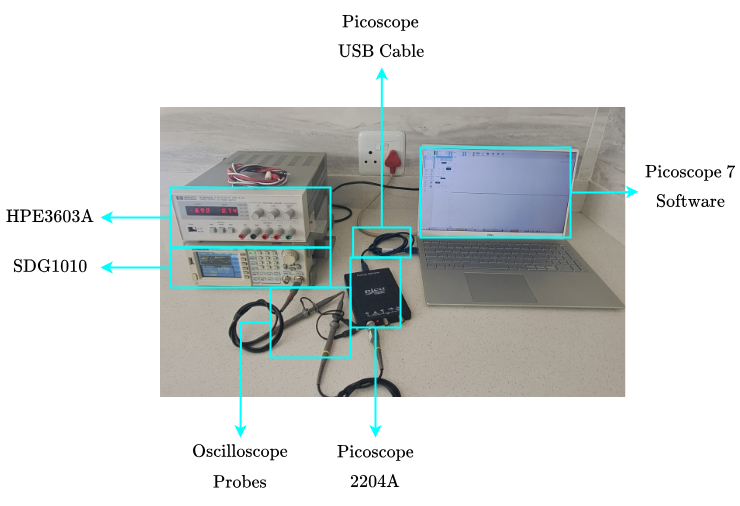
\includegraphics[width=1.1\linewidth]{Figures/Results/hp141t-test-environment.png}
			\caption{Test environment for waveform generation of HP141T auxiliary outputs.}
			\label{fig:hp141t-test-environment}
		\end{subfigure}%
		\begin{subfigure}{.33\textwidth}
			\centering
			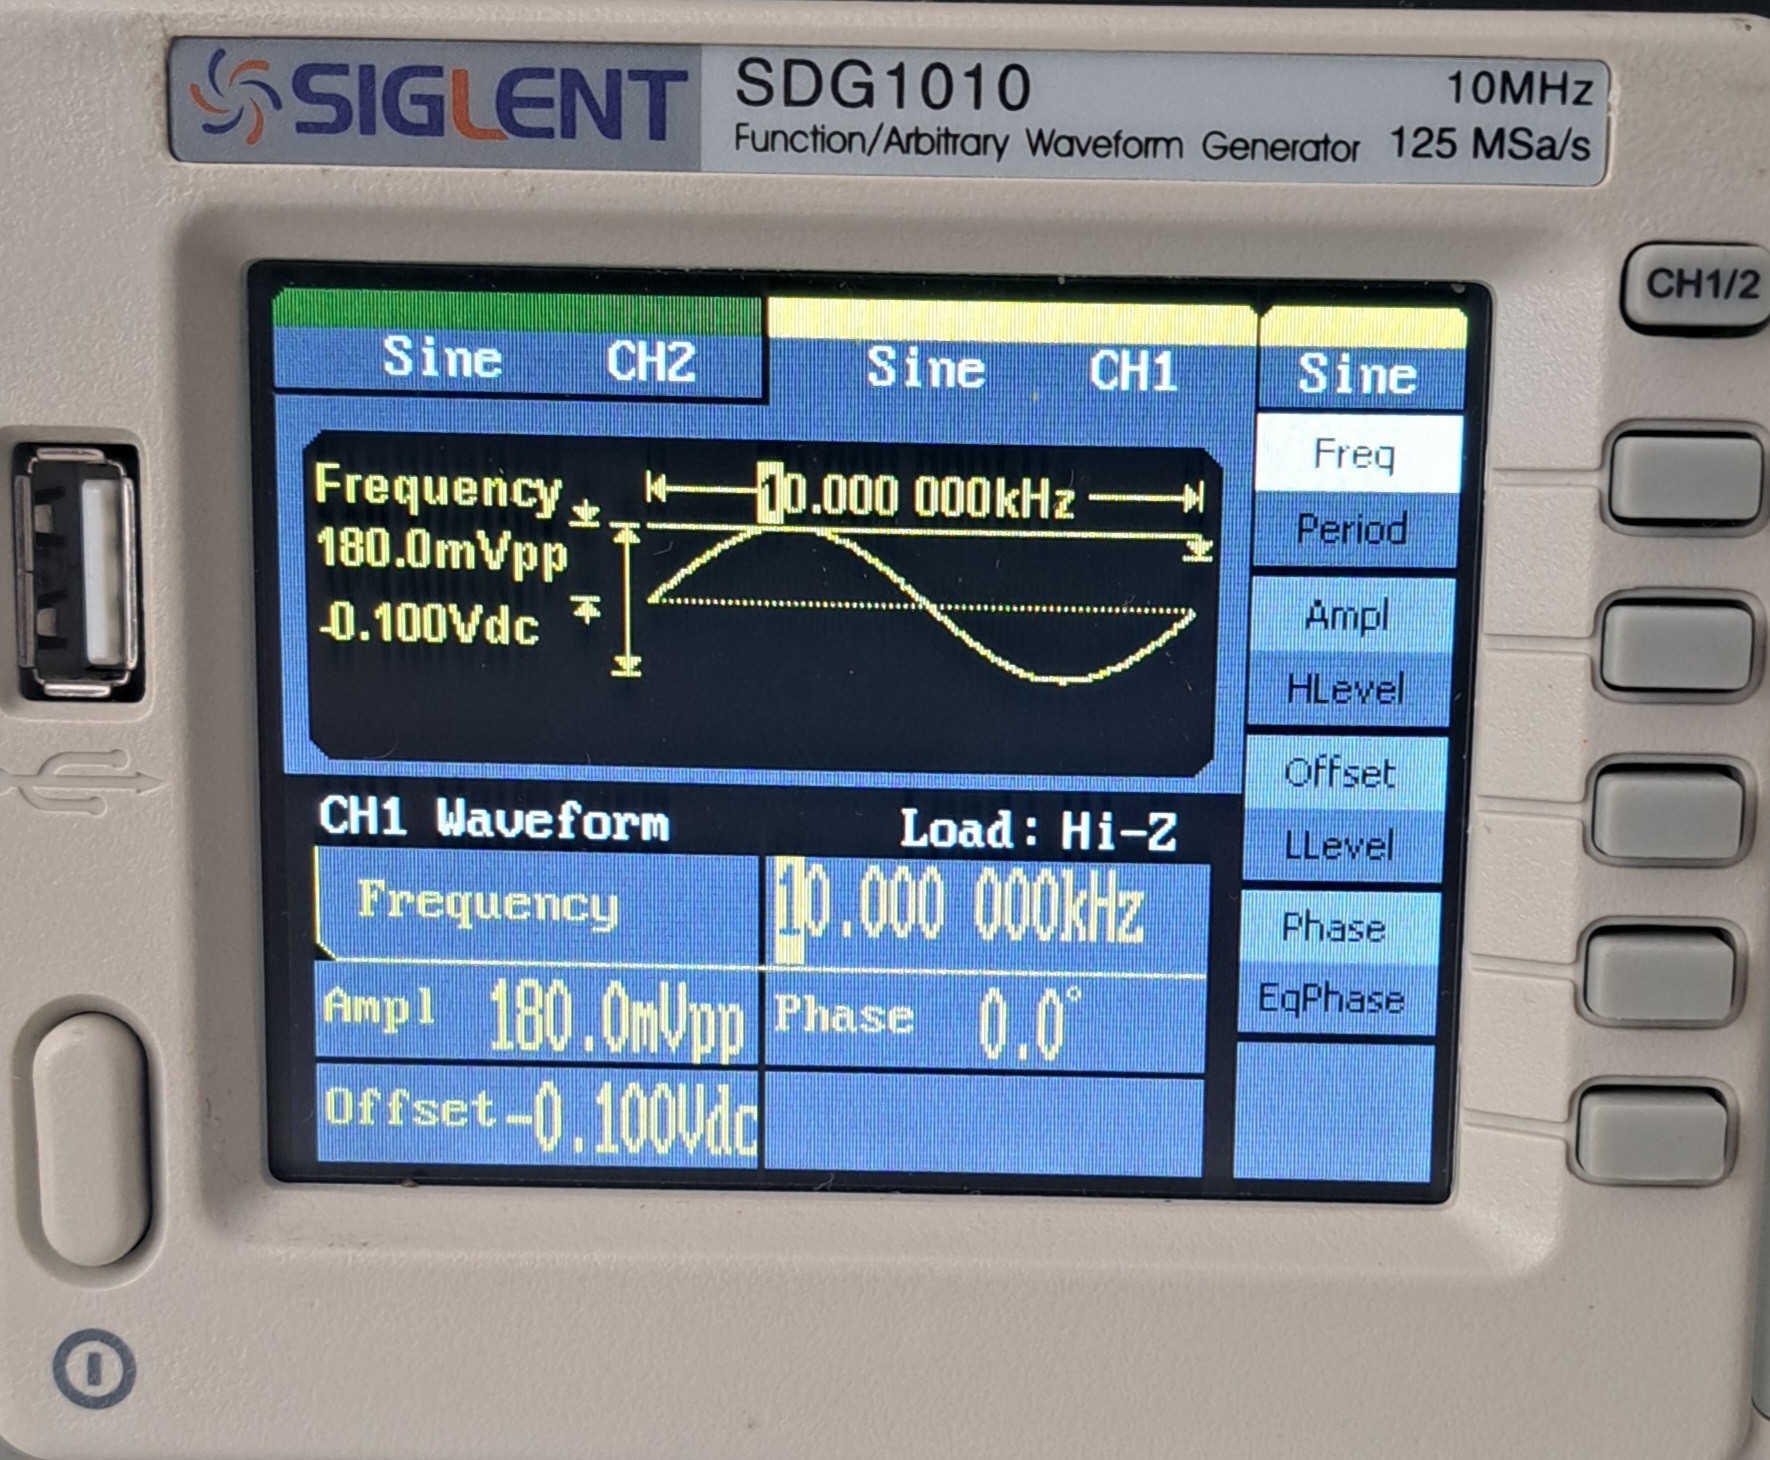
\includegraphics[width=0.55\linewidth]{Figures/Results/hp141t-002Vpp-SDG-shot}
			\caption{Example of how the vertical output was setup on the waveform generator.}
			\label{fig:hp141t-002Vpp-SDG-shot}
		\end{subfigure}
		\begin{subfigure}{.33\textwidth}
			\centering
			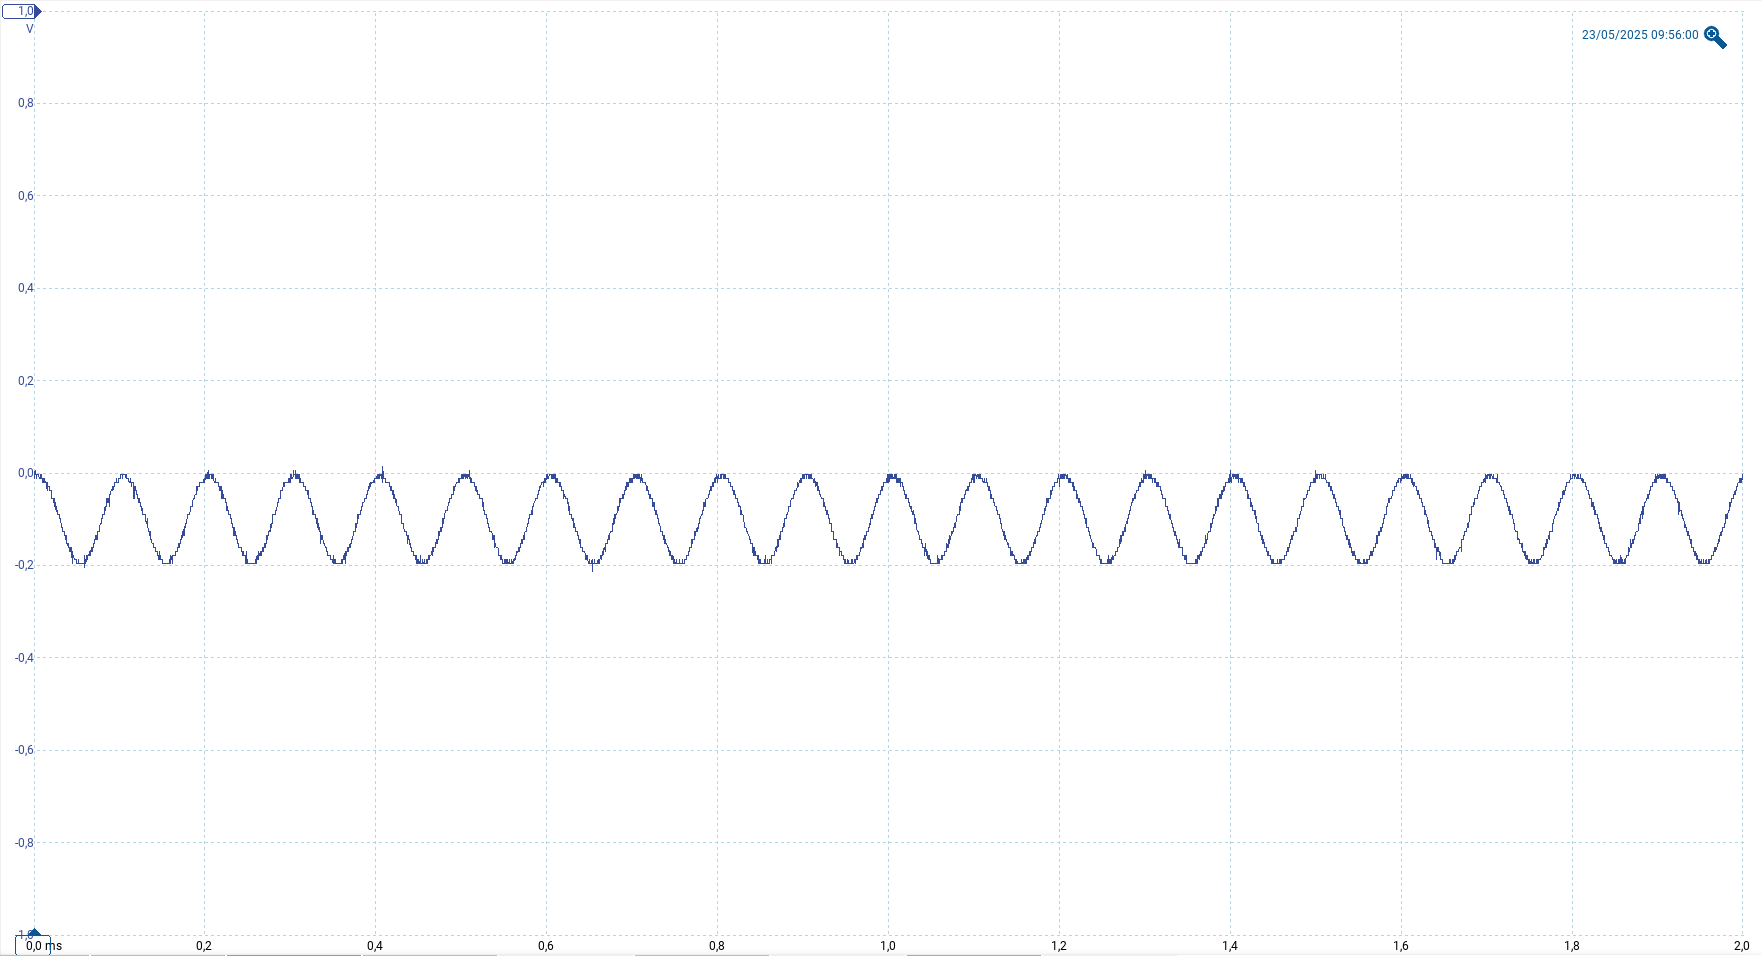
\includegraphics[width=1.0\linewidth]{Figures/Results/hp141t-02Vpp-10kHz}
			\caption{Picoscope display of the waveform generator's $\SI{180}{\milli\volt}_{pp}$ ($\SI{10}{\kilo\hertz}$) output setup shown alongside.}
			\label{fig:hp141t-002Vpp}
		\end{subfigure}
		\caption{Test environment for the approximating outputs of the HP8552B plug-in section.}
		\label{fig:hp141t-test-hardware}
	\end{figure} 

	A sinusoidal waveform was used to approximate the vertical output of the HP141T using the SDG1010 waveform generator as seen in the figures in \ref{fig:hp141t-test-hardware}. A sinusoidal waveform was found to be suitable for testing because it enabled fine adjustments of the amplitude and frequency with accurate measurements. 
	
	The characteristics of the approximate vertical output were analyzed in the Picoscope 7 software, as depicted in figure \ref{fig:hp141t-002Vpp} which shows a display of time domain characteristics of the wave generator output. Together, the results from the Picoscope software in figure \ref{fig:hp141t-test-hardware} showed that to generate the vertical output signal with a peak voltage at $\SI{0}{\volt}$, a minimum voltage of $-\SI{200}{\milli\volt}$, and frequency of $\SI{10}{\kilo\hertz}$, the amplitude of the wave from the SDG1010 should be set to $\SI{180}{\milli\volt}$ with an offset of $-\SI{100}{\milli\volt}$. This implied that the peak-to-peak voltage of the waveform from the SDG1010 deviated from the true value by $10\%$.
	
	Further investigation into the deviation of the output peak-to-peak voltage from the value set on the waveform generator was conducted by performing measurements with different voltage between $\SI{0}{\milli\volt}$ and $-\SI{0.8}{\volt}$. The results from the investigation are illustrated in figure \ref{fig:hp141t-vert-test-results} and summarized in table 4.1. 
	
	\begin{figure}[h!]
		\centering
		\begin{subfigure}{.32\textwidth}
			\centering
			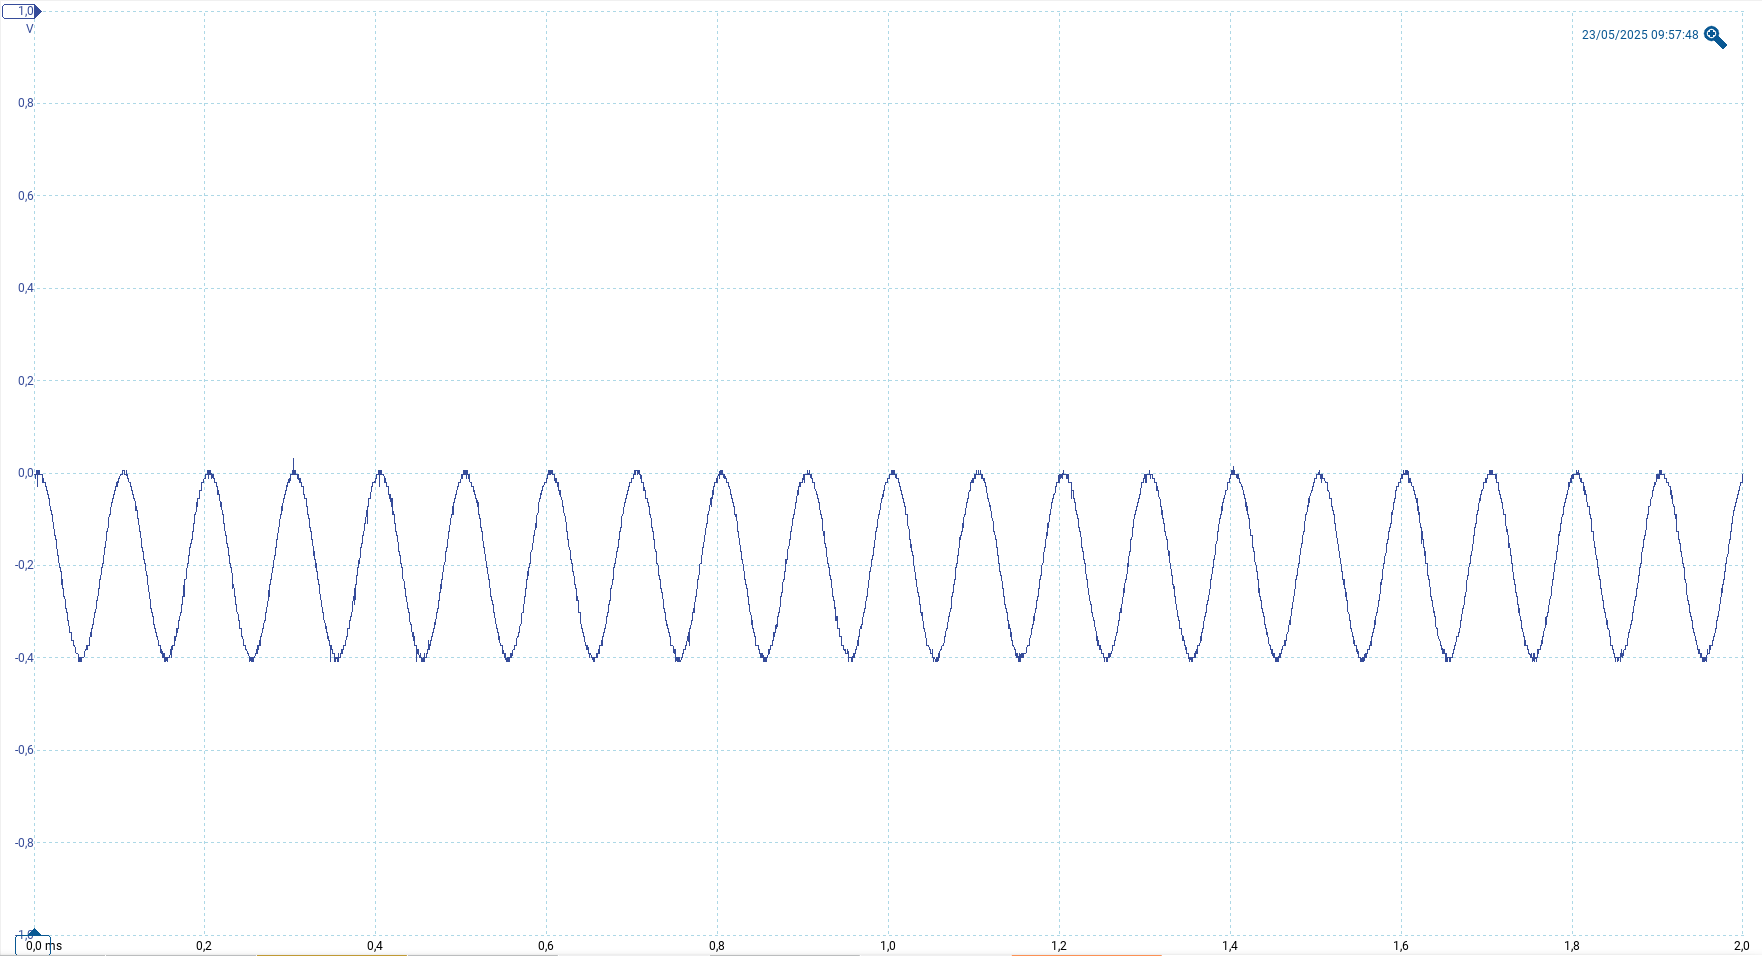
\includegraphics[width=0.95\linewidth]{Figures/Results/hp141t-004Vpp-10kHz}
			\caption{A peak-to-peak output voltage of $\SI{400}{\milli\volt}$ for an input waveform set to $\SI{180}{\milli\volt}$ at $\SI{10}{\kilo\hertz}$.}
			\label{fig:hp141t-04Vpp-10kHz}
		\end{subfigure}%
		\begin{subfigure}{.32\textwidth}
			\centering
			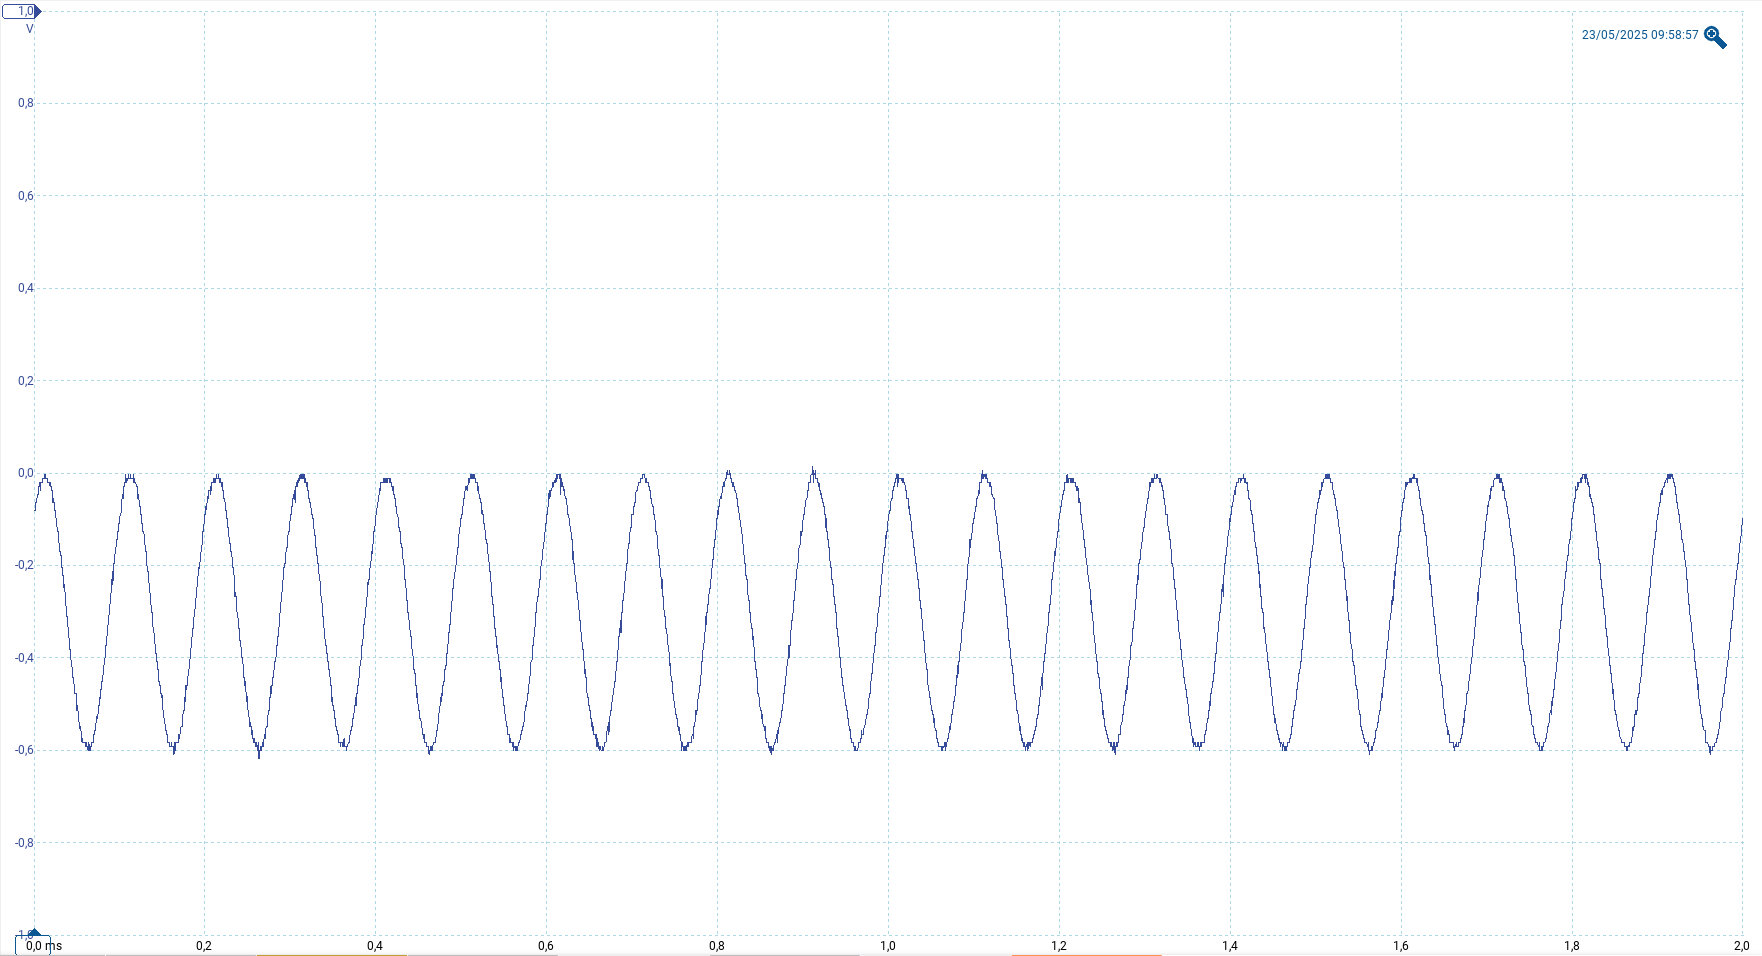
\includegraphics[width=0.95\linewidth]{Figures/Results/hp141t-006Vpp-10kHz}
			\caption{A peak-to-peak output voltage of $\SI{600}{\milli\volt}$ for an input waveform set to $\SI{260}{\milli\volt}$ at $\SI{10}{\kilo\hertz}$.}
			\label{fig:hp141t-006Vpp-result}
		\end{subfigure}
		\begin{subfigure}{.32\textwidth}
			\centering
			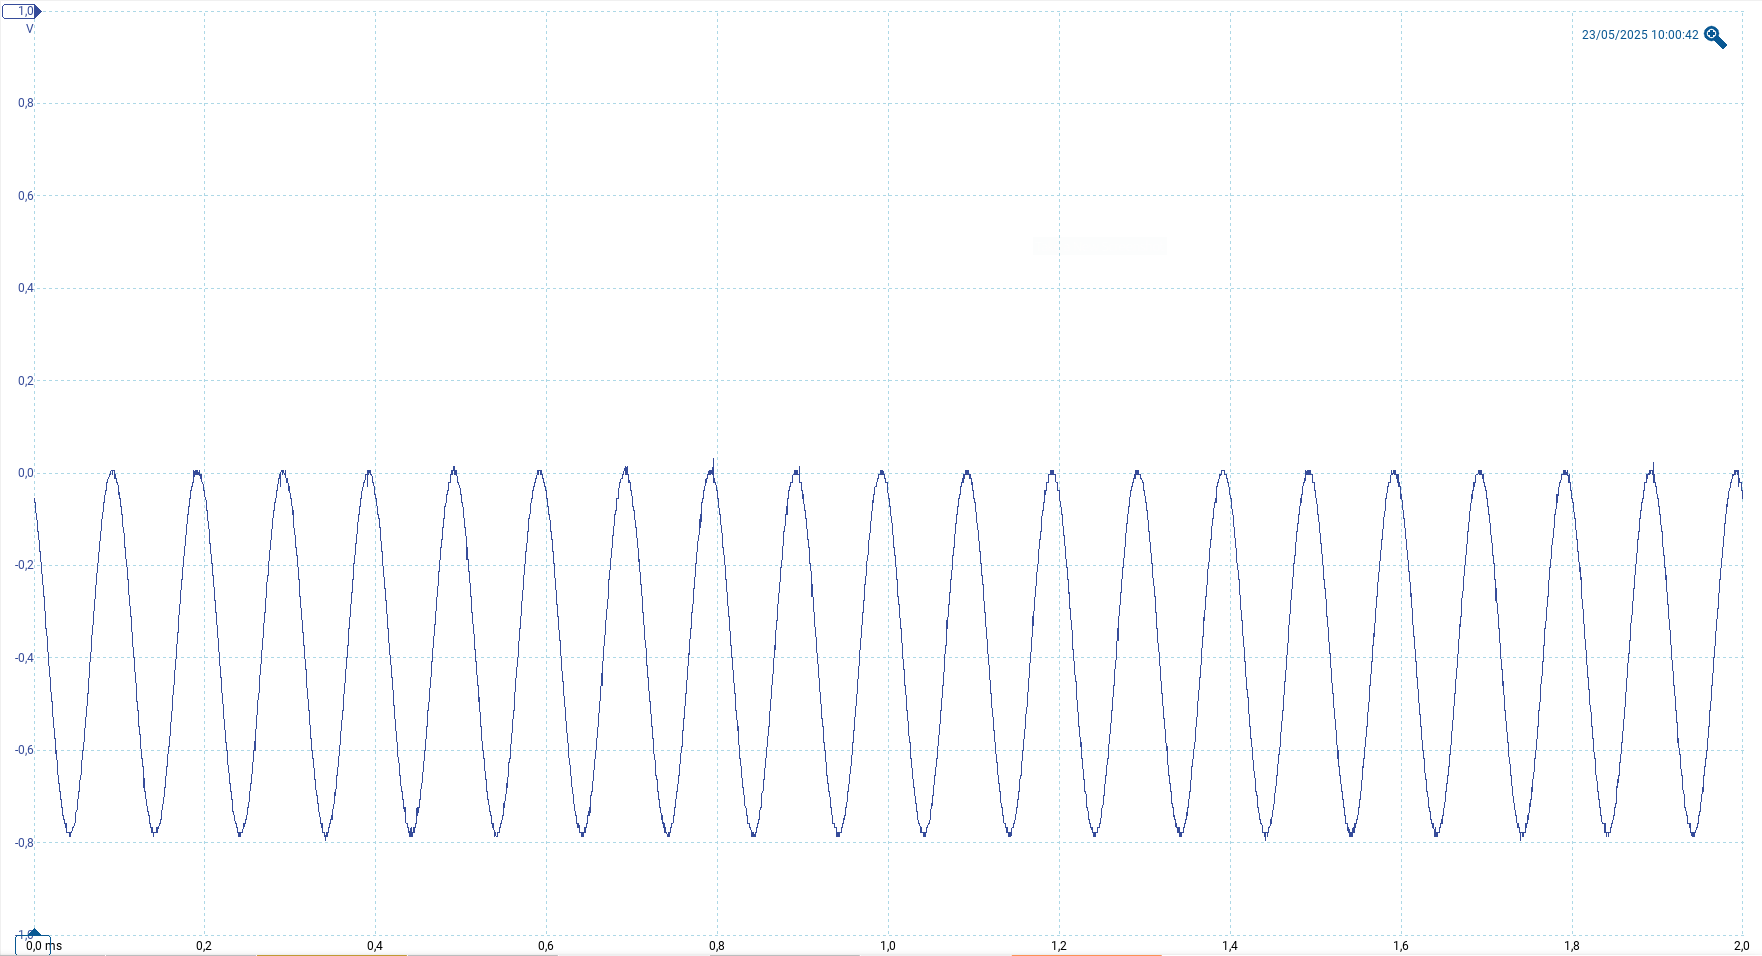
\includegraphics[width=0.95\linewidth]{Figures/Results/hp141t-008Vpp-10kHz}
			\caption{A peak-to-peak output voltage of $\SI{800}{\milli\volt}$ for an input waveform set to $\SI{320}{\milli\volt}$ at $\SI{10}{\kilo\hertz}$.}
			\label{fig:hp141t-008Vpp-result}
		\end{subfigure}
		\caption{Results from the investigation of the relationship between the vertical output's peak-to-peak voltage settings on the SDG1010 and the measured peak-to-peak voltage in Picoscope 7. The frequency and phase were maintained at constant values of $\SI{10}{\kilo\hertz}$ and $\SI{0}{\degree}$, respectively.}
		\label{fig:hp141t-vert-test-results}
	\end{figure} 
	
	In each case, an adjustment was required setup the SDG1010 such that the output has negative values between $\SI{0}{\volt}$ and $-\SI{0.800}{\volt}$. Results also showed that smaller voltage ranges between $\SI{0}{\milli\volt}$ and $-\SI{0.4}{\volt}$ were more susceptible to noise. This was observed from the increase in the smoothness of the displayed output in the Picoscope \acrshort{ui}.
	
	\begin{table}[ht!]
		\centering
		\label{tab:hp141t-vert-test-results}
		\begin{tabular}{|m{5em}|m{8em}|m{8em}|m{8em}|m{8em}|}
			\hline
			\textbf{Assessment ID} & \textbf{Measured Peak-to-Peak Value} (V)	& \textbf{Set Value} (V) & \textbf{Set Offset} (V) & \textbf{Measurement Accuracy} ($\%$)\\
			\hline
			1 & $0.202$ & $0.197$ & $-0.100$ & $2.5$\\
			\hline
			2 & $0.398$ & $0.390$ & $-0.200$ & $2.1$\\
			\hline
			3 & $0.600$ & $0.576$ & $-0.300$ & $4.2$\\
			\hline
			4 & $0.800$ & $0.765$ & $-0.400$ & $4.6$\\
			\hline
		\end{tabular}
		\caption{Investigative results of the relationship between the vertical output's peak-to-peak voltage settings on the SDG1010 and the measured peak-to-peak voltage in Picoscope 7. The frequency and phase were maintained at constant values of $\SI{10}{\kilo\hertz}$ and $\SI{0}{\degree}$, respectively.}
	\end{table}
	The table shows that the percentage accuracy of the test environment for setting up the vertical output decreases as the approximated value approaches a maximum value of $-\SI{0.800}{\volt}$. The measurements were taken starting from a peak-to-peak voltage of $\SI{0.2}{\volt}$. The standard deviation in the measured results was found to be $0.223$ and the standard deviation in the set peak-to-peak values was $0.211$.
	
	Given that some spectrum consist of multiple frequency components, a noisy signal was used to approximate the vertical output more closely as shown in figure \ref{fig:noisy-vertical}. The vertical output from the original HP141T system was expected to fluctuate rapidly with a frequency of up to $\SI{300}{\kilo\hertz}$. To approximate this behaviour using the SDG1010, the standard deviation of the generated Gaussian noise was set to $\SI{136.2}{\milli\volt}$ and the mean was set to $-\SI{360}{\milli\volt}$. 
	\begin{figure}[ht!]
		\centering
		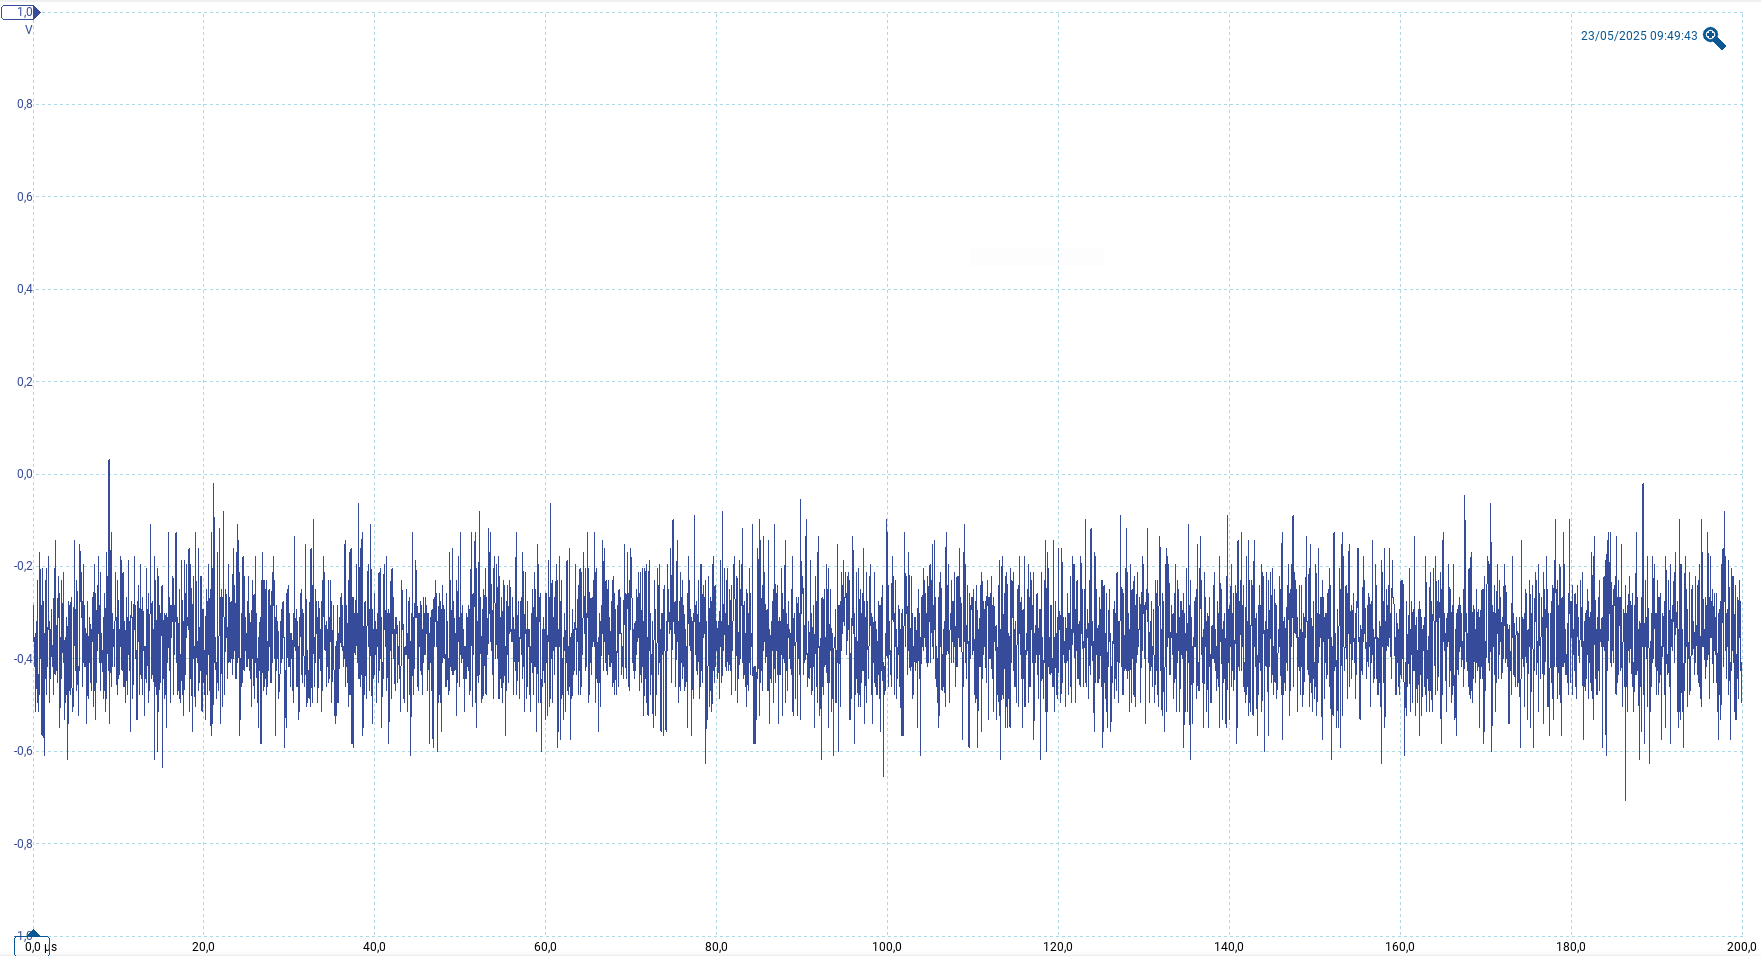
\includegraphics[width=0.64\linewidth]{Figures/Results/hp141t-noisy}
		\caption{Showing approximation of the vertical output with a noisy signal from the wave generator.}
		\label{fig:noisy-vertical}
	\end{figure} 
	
	The horizontal output was also approximated using a waveform generator. However, the sawtooth shape of the signal was approximated using the ramp function on the SDG1010 signal generator. The resultant shape of the output waveform, depicted in figure \ref{fig:hp141t-sawtooth-test}, did not match the desired shape of the HP8552B, as shown in figure \ref{fig:hp8552b-sawtooth}. Therefore, the approximated horizontal output from the SDG1010 could only be used to assess the behaviour of subsequent systems with respect to the amplitude. Although the results of the scan time were considered, the output from the waveform generator does not accurately represent the timing-behaviour of the system when the original HP141T horizontal output is used.
	
	\begin{figure}[h!]
		\centering
		\begin{subfigure}{.48\textwidth}
			\centering
			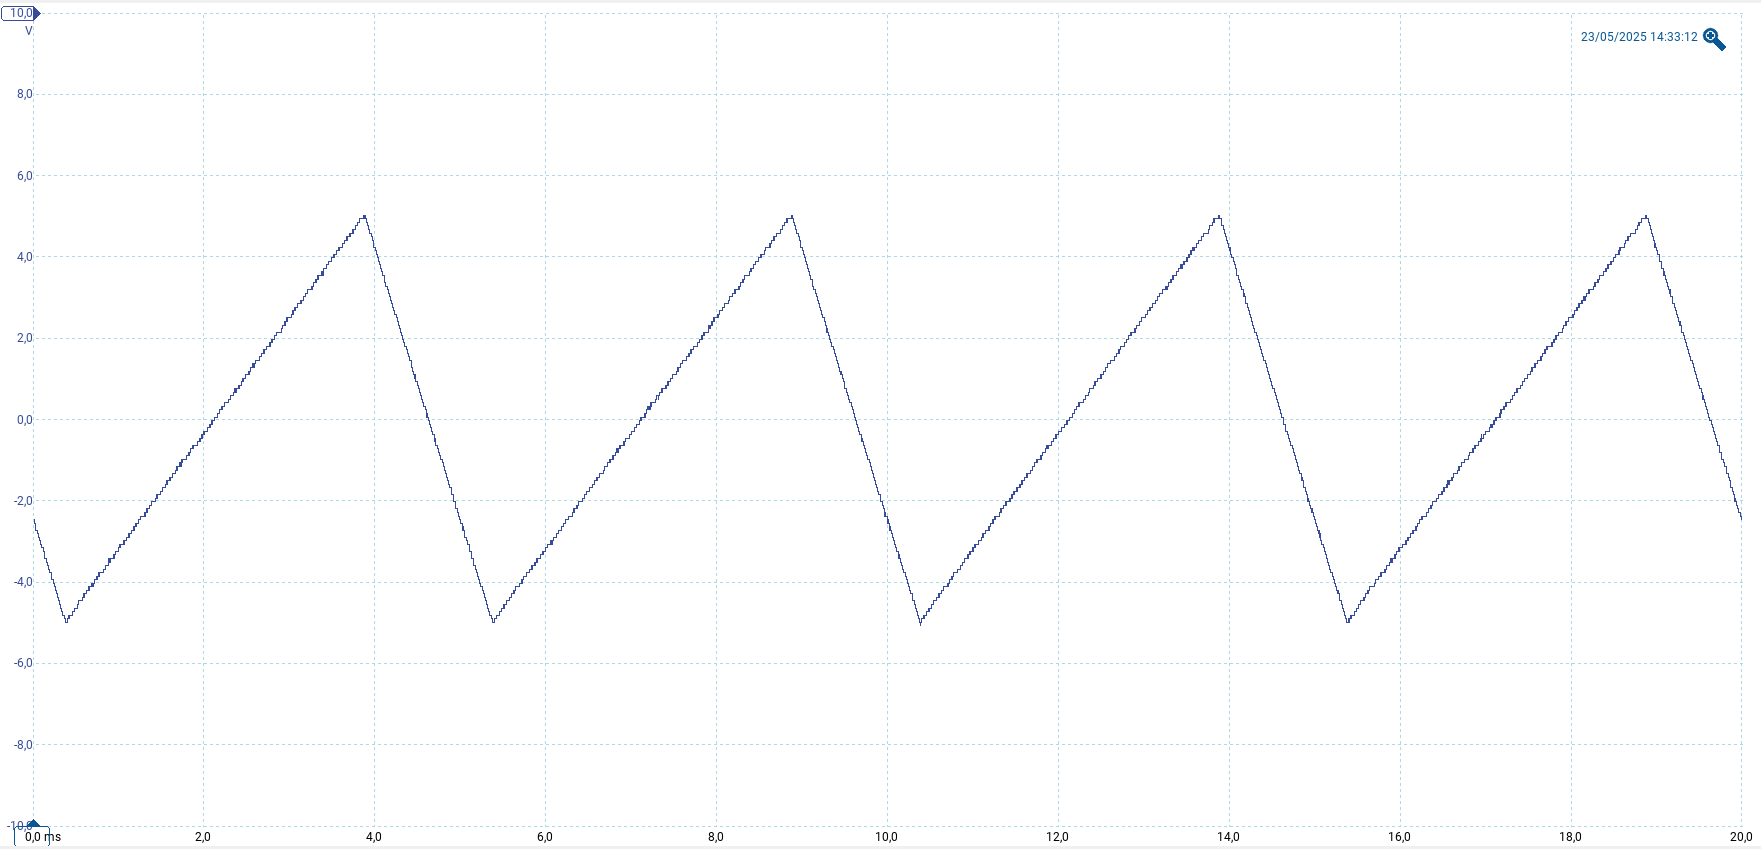
\includegraphics[width=0.95\linewidth]{Figures/Results/hp141t-sawtooth-test}
			\caption{Approximation results of the HP141T's sawtooth scan output using a ramp waveform generated by the SDG1010. The shape of the wave did not approximate the shape of the HP141T output.}
			\label{fig:hp141t-sawtooth-test}
		\end{subfigure}%
		\begin{subfigure}{.48\textwidth}
			\centering
			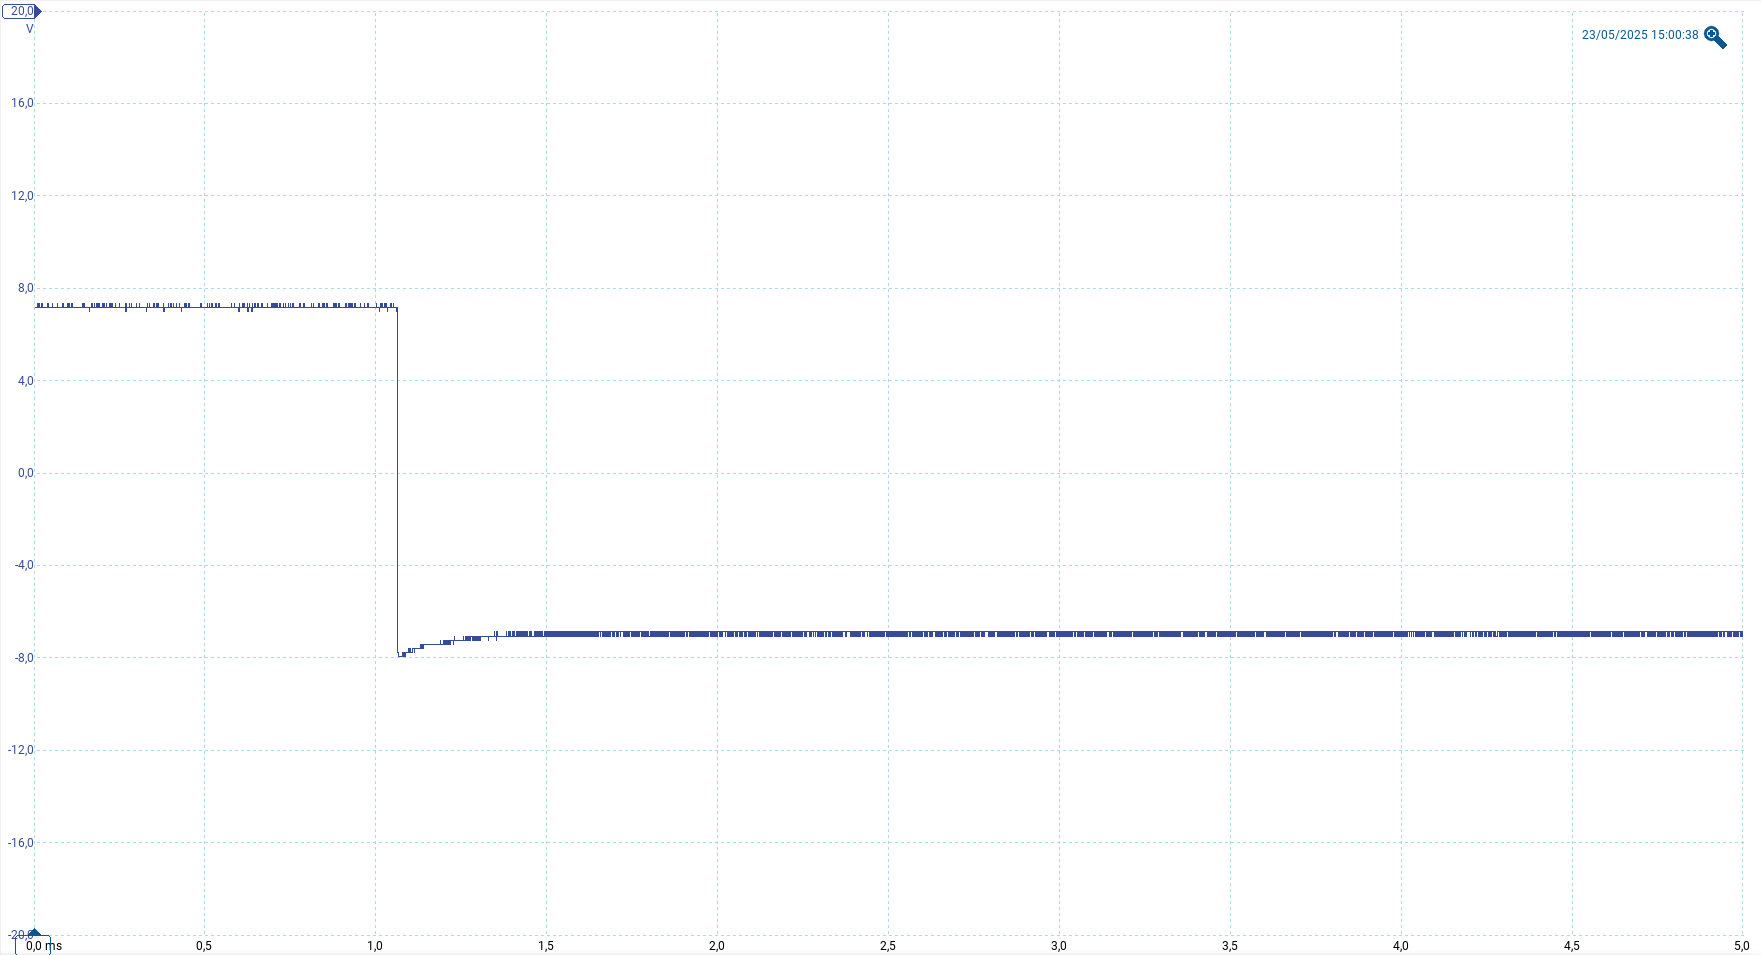
\includegraphics[width=0.95\linewidth]{Figures/Results/hp141t-penlift-test}
			\caption{The pen-lift-output could not be achieved using the SDG1010 as the voltage range was outside of the desired $[\SI{0}{\volt}, \SI{14}{\volt}]$ interval.}
			\label{fig:hp141t-penlift-test}
		\end{subfigure}
		\caption{Test results of the approximated values of the horizontal and pen-lift outputs of the original HP141T system obtained using the Siglent SDG1010.}
		\label{fig:hp141t-horpen-test-results}
	\end{figure} 

	Attempts to approximate the pen-lift output using a square wave generated by the SDG1010 yielded the signal as shown in figure \ref{fig:hp141t-penlift-test}. The maximum value of the output was $\SI{7}{\volt}$ and the minimum value was $\SI{-7}{\volt}$ when the waveform generator was configured to produce a peak-to-peak voltage of $\SI{14}{\volt}$. Given that the SDG1010's maximum allowable offset is $\SI{4.999}{\volt}$, the square wave could not be shifted to fit the desired range of the pen-lift output between $\SI{0}{\volt}$ and $\SI{14}{\volt}$. Therefore, an accurate approximation of the original \acrshort{sa}'s pen-lift output was not achievable using the SDG1010. 
	
	Overall, the unit tests for verifying voltage levels of outputs from the original HP141T system could not be performed directly on the device. However, the results show that the vertical output can be approximated using the SDG1010 with satisfactory accuracy. The results also verify that the Picoscope is a suitable test tool for the system.
	
	\section{HP141T Emulator Subsystem Test Results}
	
	This section presents the results of unit testing the HP141T Emulator \acrshort{pcb}, which is responsible for signal emulation and waveform generation. The tests focus on validating the behavior of the analog outputs (vertical, horizontal, and pen-lift signals) against expected electrical characteristics described in the methodology. Each test verifies waveform amplitude, frequency range, and functional timing to ensure compatibility with downstream processing.
	
	Construction of the HP141T Emulator was completed as shown in figure \ref{fig:emulator-hardware}. The circuit was connected to the HP-E3630A power supply as a required dual rail power supply. The \acrshort{led} associated with the power rail turned on, indicating that electricity was flowing through the circuit to the ground plane.
	
	\begin{figure}[ht!]
		\centering
		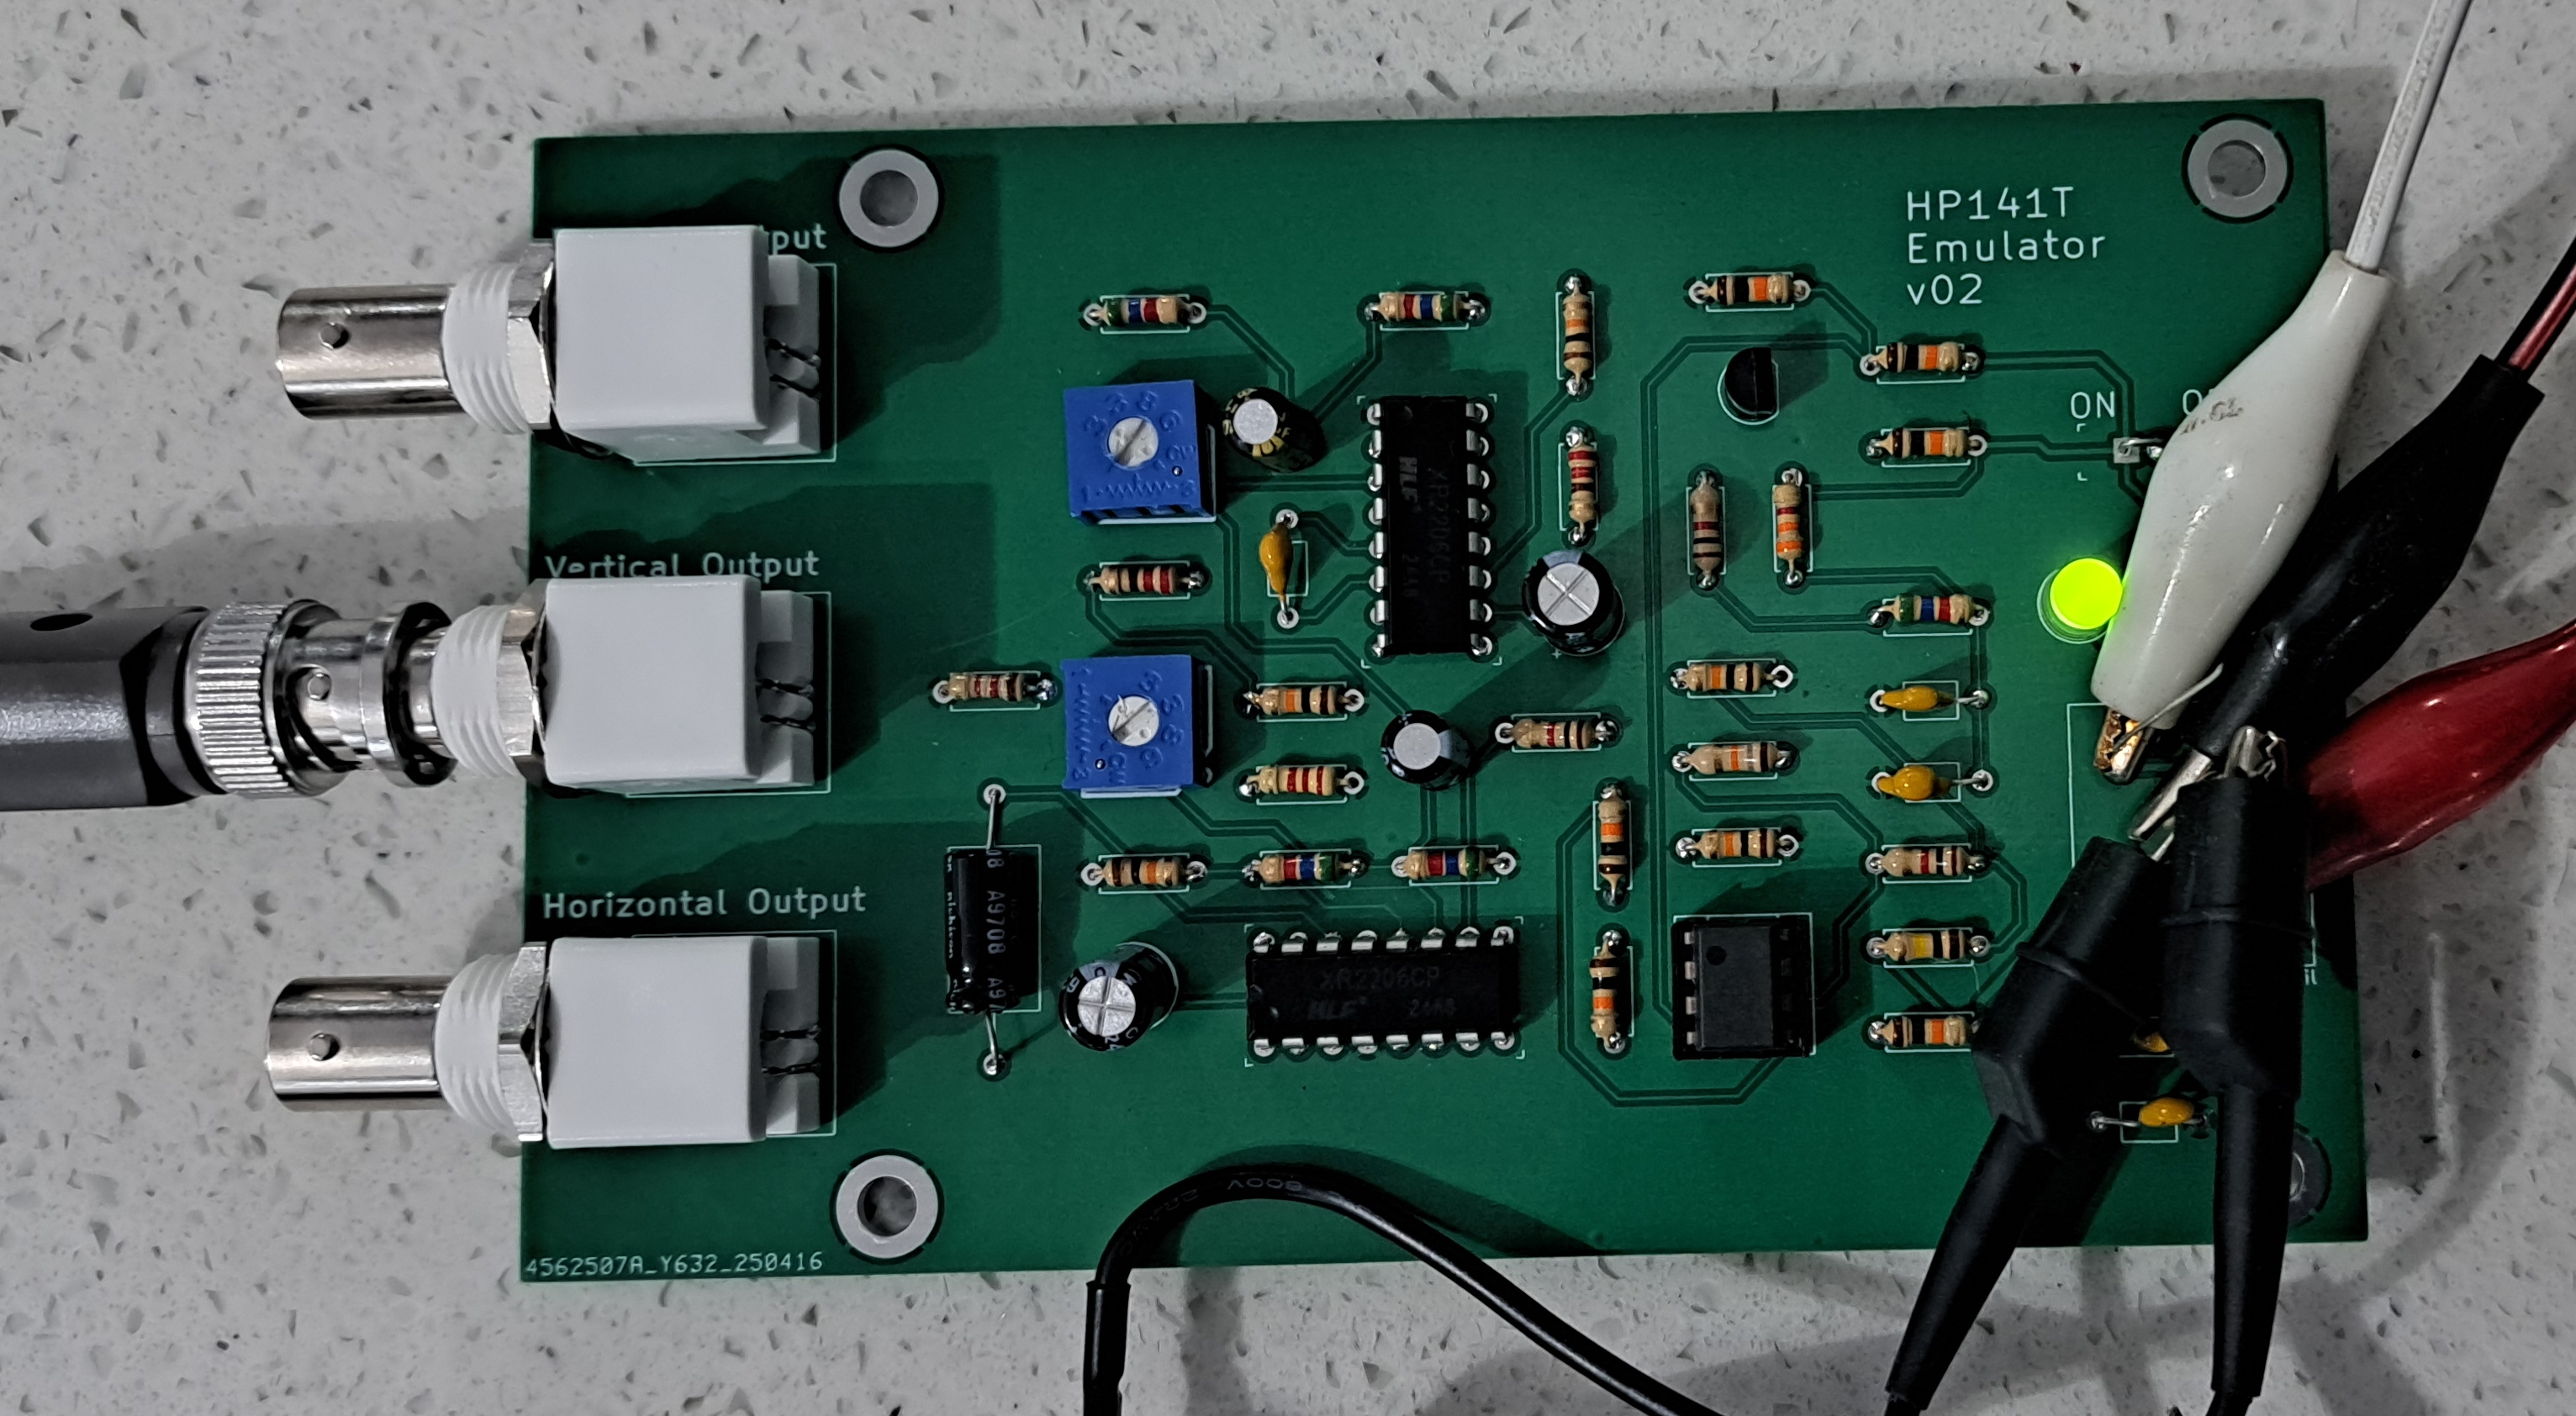
\includegraphics[width=0.55\linewidth]{Figures/Results/emulator-hardware}
		\caption{Showing construction of the HP141T Emulator and connection to the HP-E3630 DC power supply. The outputs of the design were collected using a oscilloscope probe connected to the Picoscope and \acrshort{bnc} adapters on the circuit.}
		\label{fig:emulator-hardware}
	\end{figure} 
	
	The graphical results depicted in figure \ref{fig:emulator-output-tests} showed that the HP141T was not operating as expected. This is accounted for by the use of different values for the resistors described in the methodology. The methodology, based on the recommended usage of the XR2206 from the datasheet, uses the E24 resistor series, whereas the available resistors in the laboratory setting belong to the E6 series. In addition, capacitance values were changed according to the availability of the capacitors in the laboratory. 
	
	\begin{figure}[h!]
		\centering
		\begin{subfigure}{.32\textwidth}
			\centering
			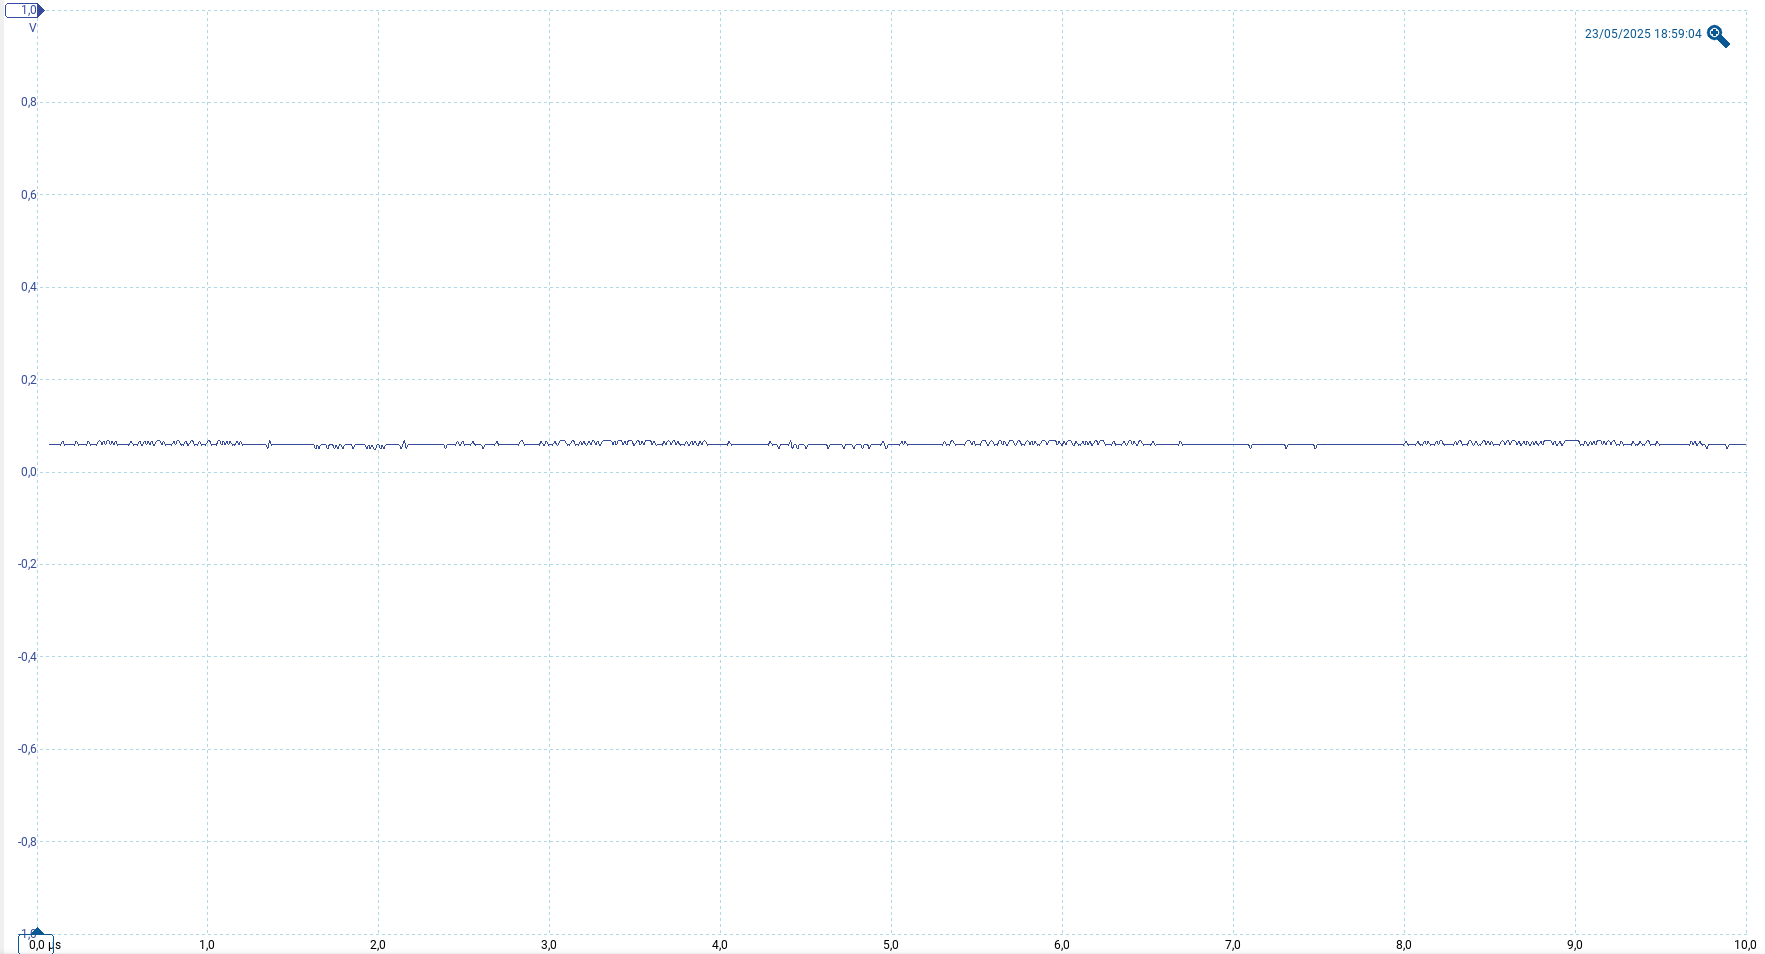
\includegraphics[width=0.95\linewidth]{Figures/Results/emulator-horizontal-output}
			\caption{Horizontal output from the HP141T Emulator.}
			\label{fig:emulator-horizontal-output}
		\end{subfigure}%
		\begin{subfigure}{.32\textwidth}
			\centering
			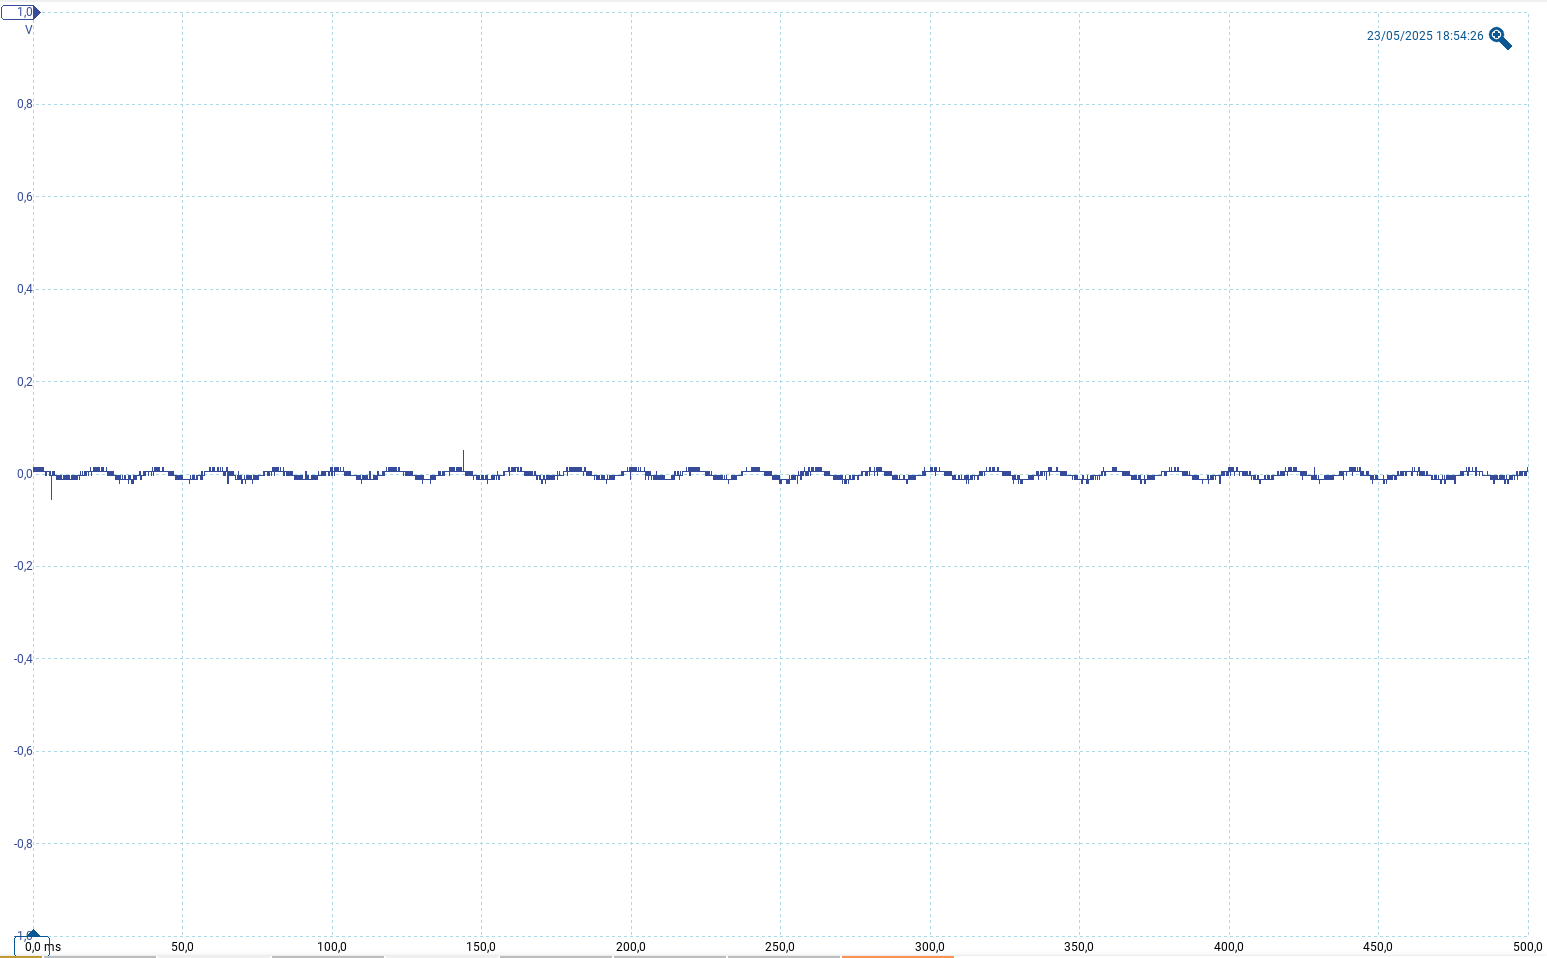
\includegraphics[width=0.95\linewidth]{Figures/Results/emulator-vertical-output}
			\caption{Vertical output from the HP141T Emulator.}
			\label{fig:emulator-vertical-output}
		\end{subfigure}
		\begin{subfigure}{.32\textwidth}
			\centering
			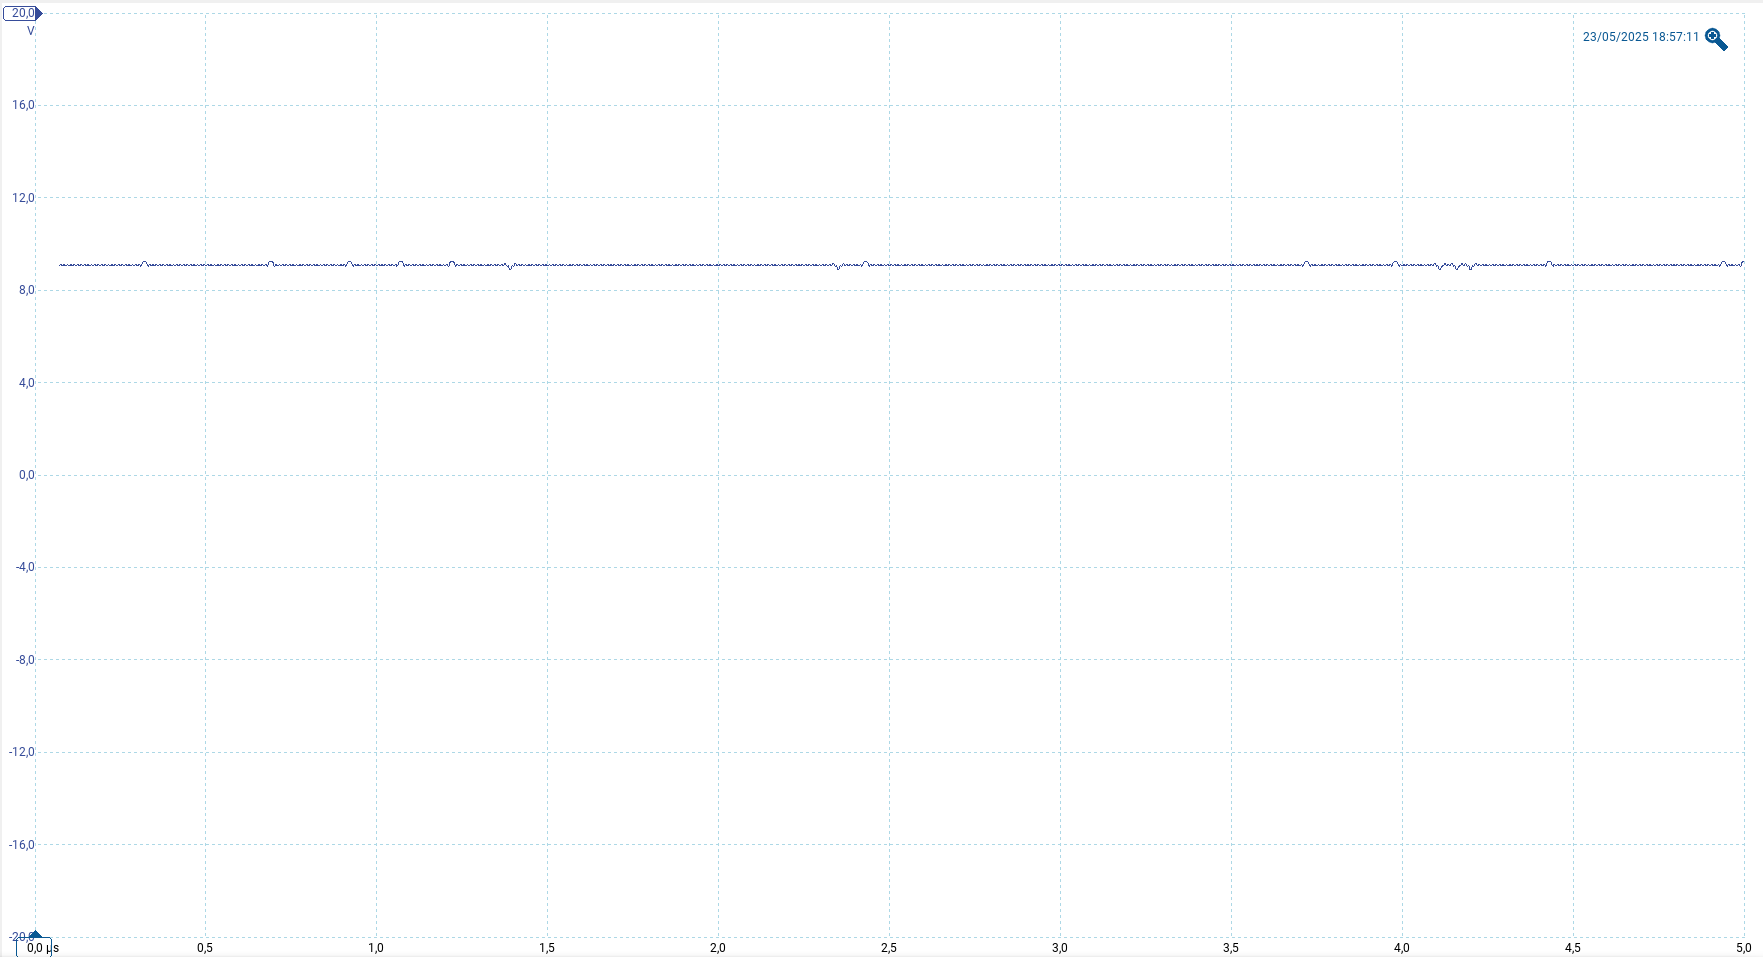
\includegraphics[width=0.95\linewidth]{Figures/Results/emulator-penlift-output}
			\caption{Pen-lift output from the HP141T Emulator.}
			\label{fig:emulator-penlift-output}
		\end{subfigure}
		\caption{Results of the HP141T Emulator indicating that the device was not operating as expected.}
		\label{fig:emulator-output-tests}
	\end{figure} 
	
	\begin{table}[ht!]
		\centering
		\begin{tabular}{|c|m{25em}|c|}
			\hline
			\textbf{ID} & \textbf{Description} & \textbf{Outcome} \\
			\hline
			UTB00 & Emulated vertical output ranges between \SI{0}{\volt} and \SI{3.0}{\volt} when a test signal is applied and viewed on the Picoscope. & Fail \\
			\hline
			UTB01 & Spectrum view confirms a \SI{10}{\hertz} component in the vertical output. & Fail \\
			\hline
			UTB02 & Horizontal output shows a sawtooth waveform ranging from \SI{-4.76}{\volt} to \SI{4.75}{\volt}, matching the scan time base configuration. & Fail \\
			\hline
			UTB03 & Pen-lift output toggles between \SI{0}{\volt} (during scan) and \SI{14}{\volt} (during retrace), synchronized with the horizontal sweep. & Fail \\
			\hline
			UTB04 & Power rails meet the expected ranges: +5V $\pm$ 0.1V, -12V $\pm$ 0.2V, and regulated +12V. & Pass \\
			\hline
		\end{tabular}
		\caption{Results of unit tests for the HP141T Emulator \acrshort{pcb}.}
		\label{tab:emulator-unit-tests}
	\end{table}
	Table \ref{tab:emulator-unit-tests} shows the outcomes of the unit tests of the HP141T Emulator. Given that the device did not operate as expected, further iterations are required to improve the performance so that the outputs resemble the HP141T's auxiliary outputs.
	\section{Signal Conditioning Subsystem Results}
	
	This section presents the measured voltage transformations and waveform fidelity at the output of the \acrshort{scs}. It compares the observed behavior against theoretical expectations based on the known input-output mappings, such as the inversion of the vertical output and scaling to the \acrshort{adc}-compatible voltage range.
	
	The \acrshort{scs} was implemented on a \acrshort{pcb} as shown in figure \ref{fig:scs-hardware} where the oscilloscope probe connected to the Picoscope is attached at vertical output of the circuit and the \acrshort{bnc}-to-\acrshort{bnc} adapter is connected to the input adapter and the signal generator. 
	
	\begin{figure}[h!]
		\centering
		\begin{subfigure}{.32\textwidth}
			\centering
			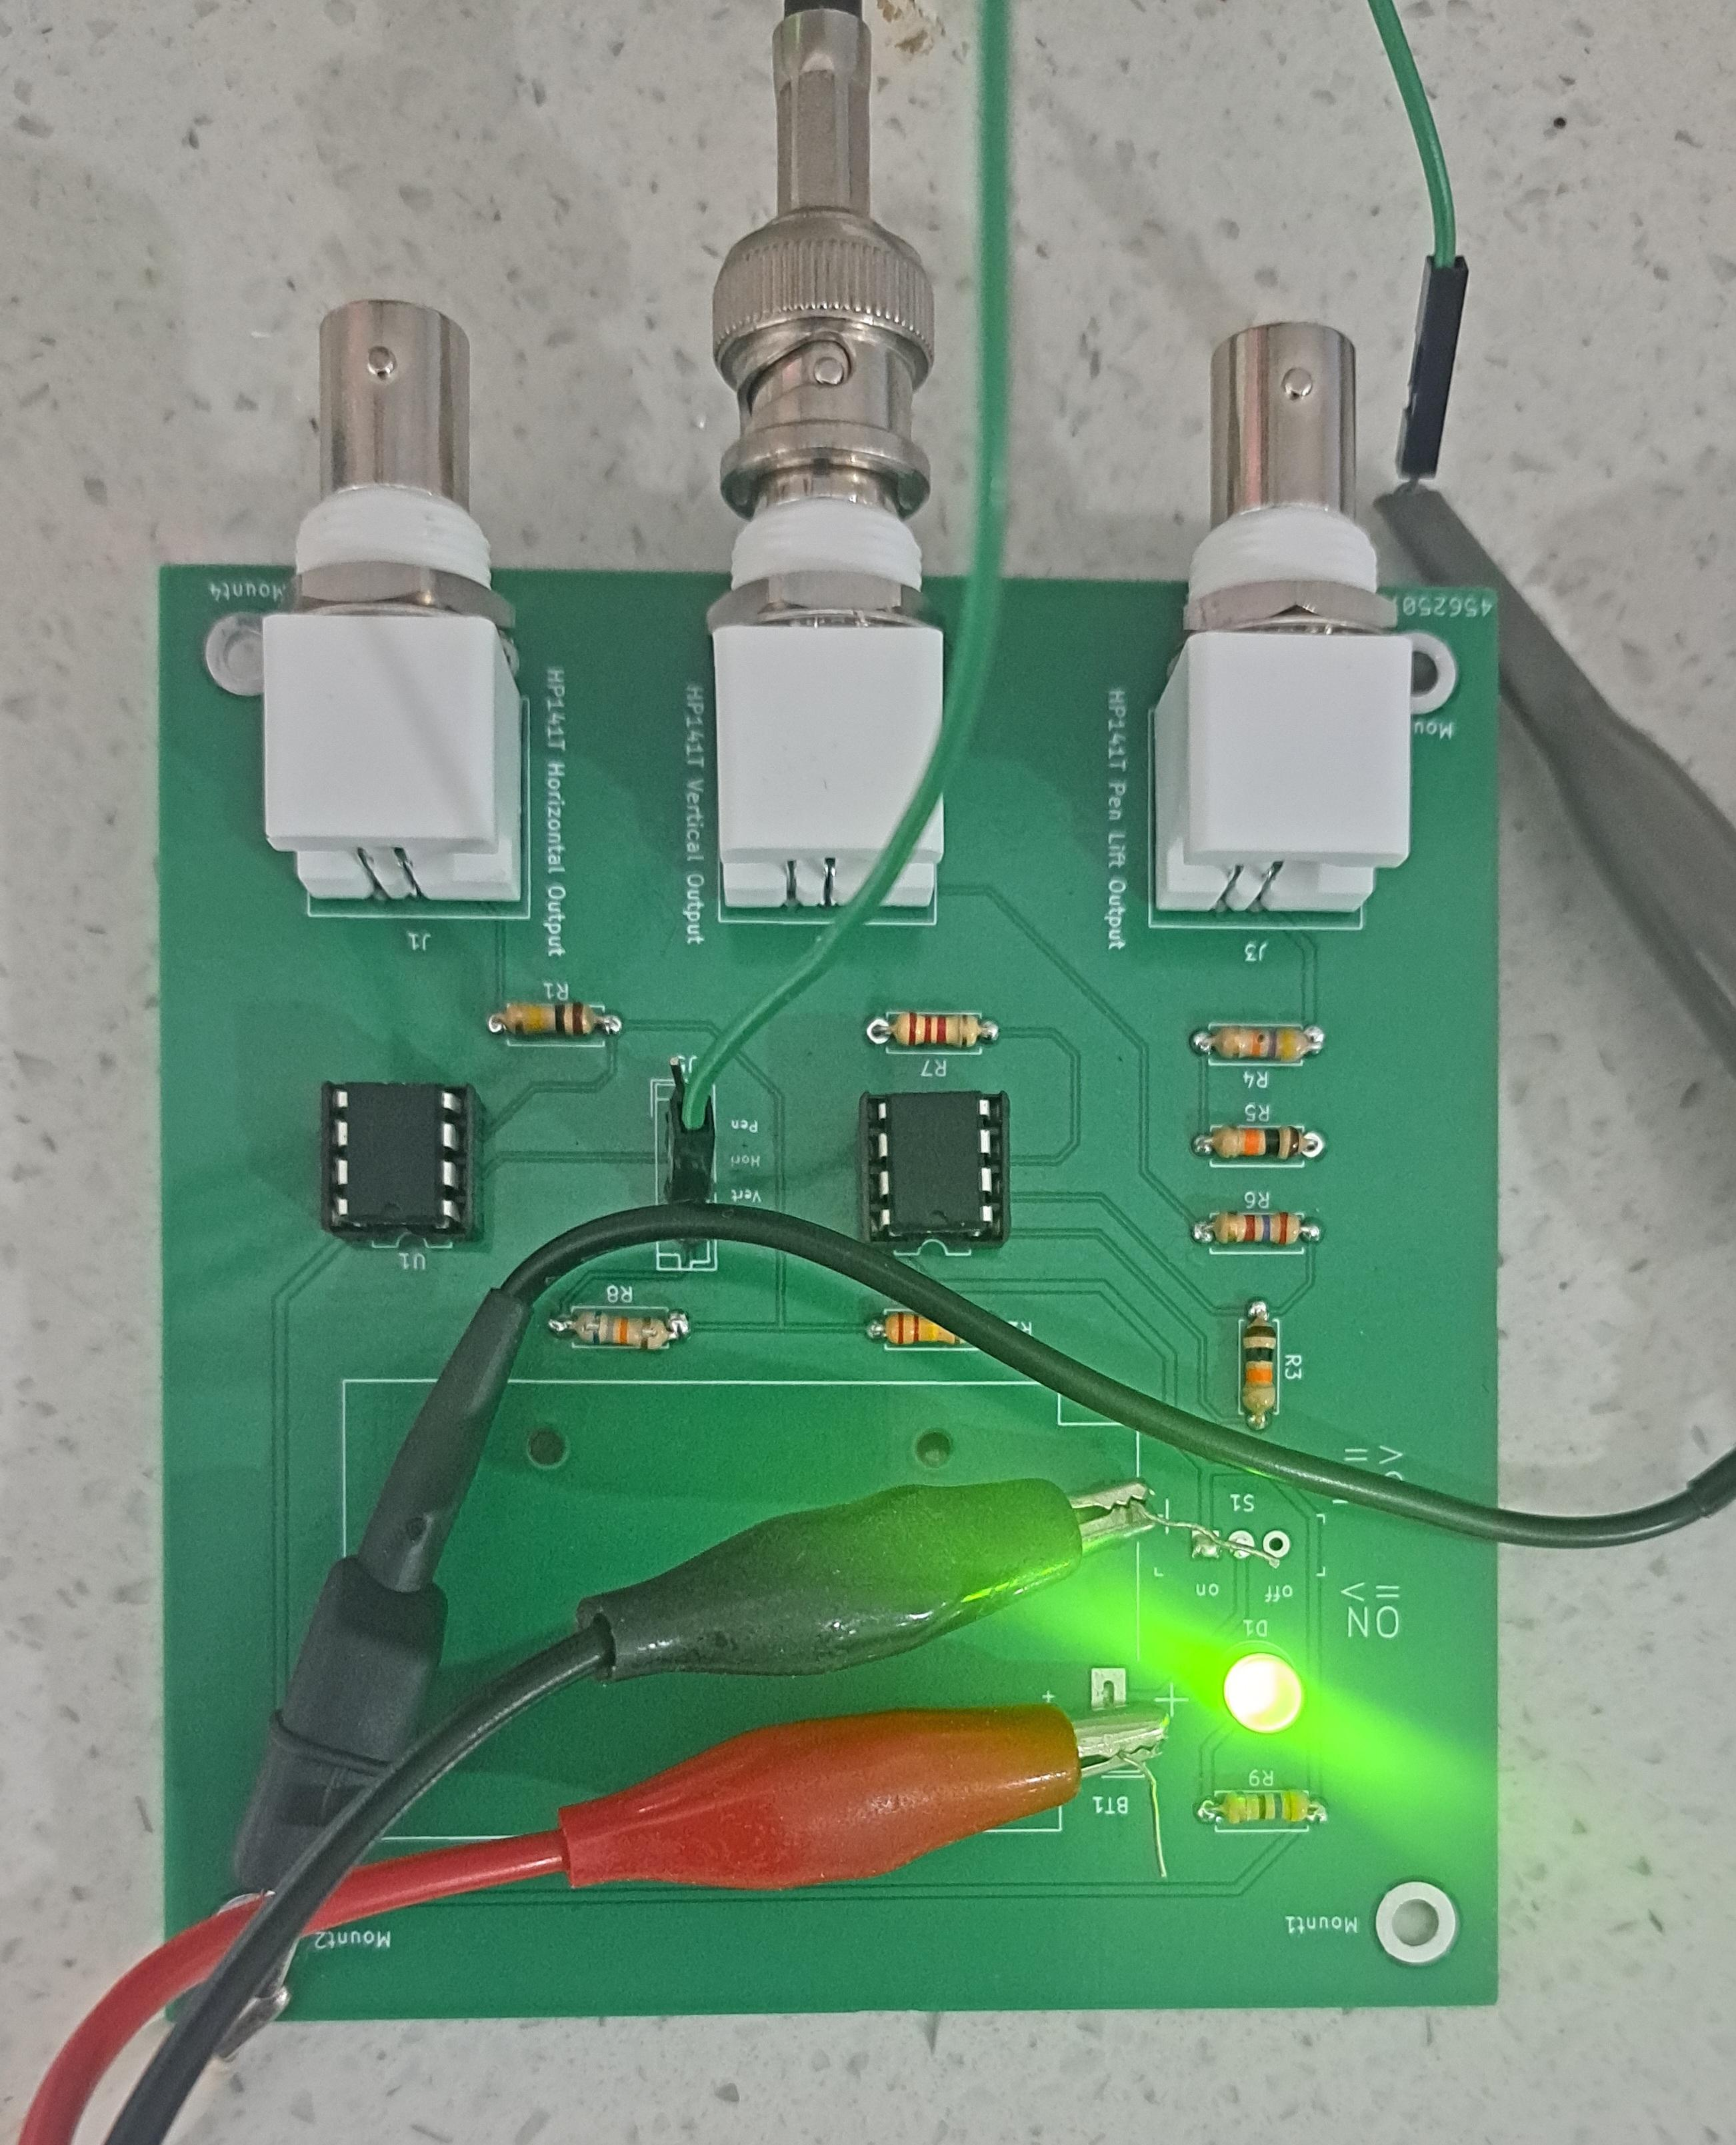
\includegraphics[width=0.95\linewidth]{Figures/Results/scs-hardware}
			\caption{\acrshort{scs} hardware implementation.}
			\label{fig:scs-hardware}
		\end{subfigure}%
		\begin{subfigure}{.32\textwidth}
			\centering
			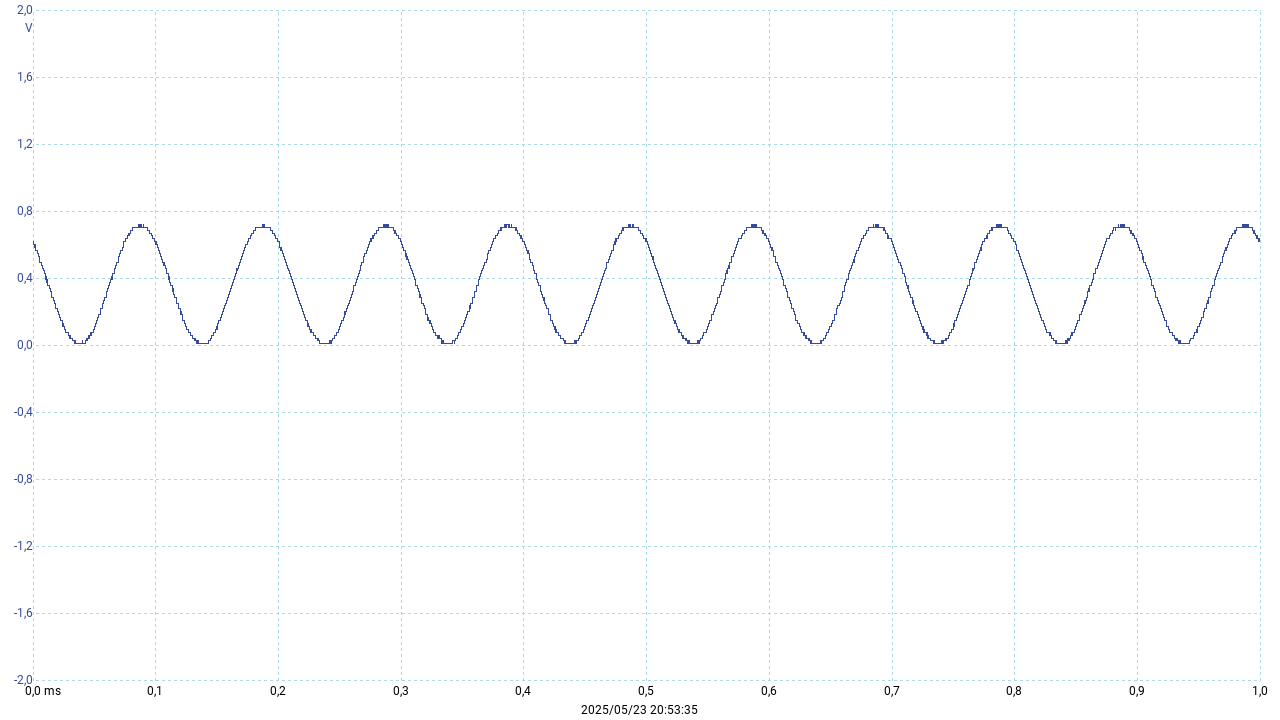
\includegraphics[width=0.95\linewidth]{Figures/Results/scs-output-02Vpp-10kHz}
			\caption{Vertical output of the \acrshort{scs} \acrshort{pcb} for a $\SI{0.2}{\volt}$ peak-to-peak voltage at $\SI{10}{\kilo\hertz}$.}
			\label{fig:scs-output-02Vpp-10kHz}
		\end{subfigure}
		\begin{subfigure}{.32\textwidth}
			\centering
			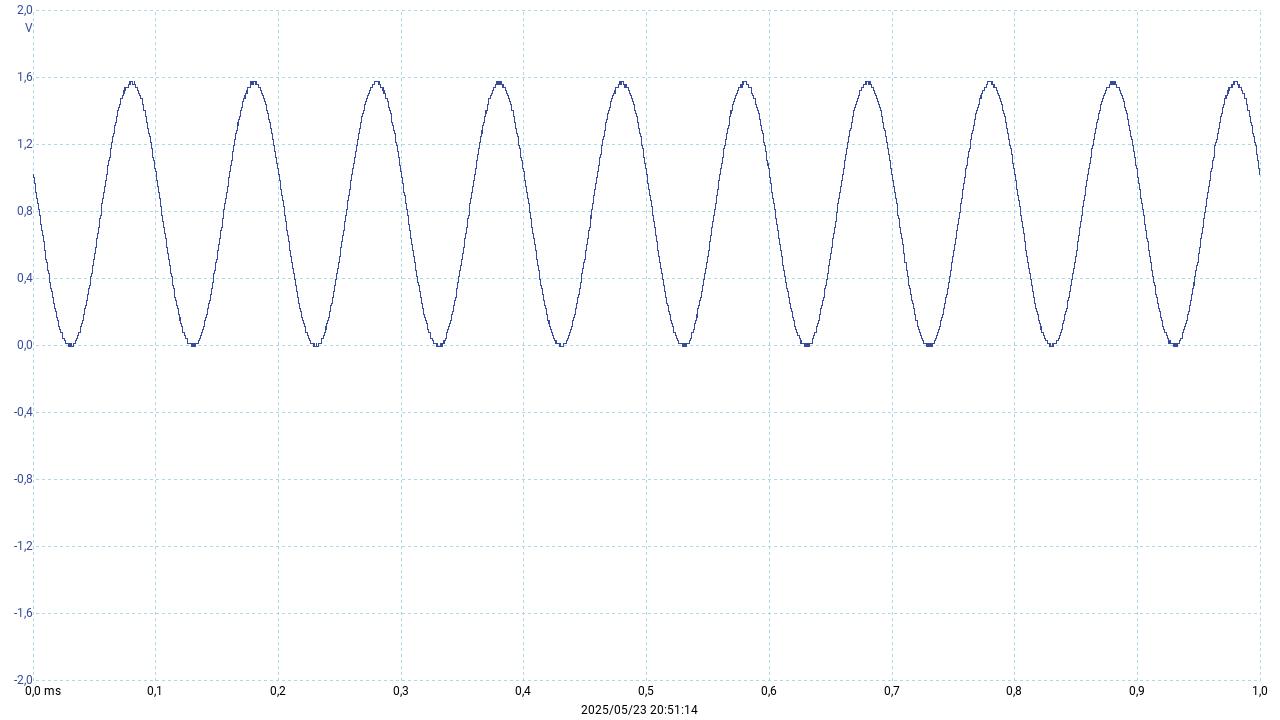
\includegraphics[width=0.95\linewidth]{Figures/Results/scs-output-04Vpp-10kHz}
			\caption{Vertical output of the \acrshort{scs} \acrshort{pcb} for a $\SI{0.4}{\volt}$ peak-to-peak voltage at $\SI{10}{\kilo\hertz}$.}
			\label{fig:scs-output-04Vpp-10kHz}
		\end{subfigure}
		\caption{Results from the implementation of the \acrshort{scs} on a \acrshort{pcb}.}
		\label{fig:scs-hardware-implementation}
	\end{figure} 
	
	The results of the \acrshort{scs} were recorded for different peak-to-peak voltages of the SDG1010-generated sinusoidal wave, while maintaining a constant $\SI{10}{\kilo\hertz}$ frequency. When the peak-to-peak voltages on the SDG1010 waveform generator were set according to the results in table \ref{tab:hp141t-vert-test-results}, the displayed output showed that the \acrshort{scs} \acrshort{pcb} was behaving as expected. For example, the output waveform in \ref{fig:scs-output-02Vpp-10kHz} shows that when an input with a peak-to-peak voltage of $-\SI{0.2}{\volt}$ was injected into the subsystem, the output of the \acrshort{scs} was $\SI{0.7}{\volt}$, showing that the subsystem adequately inverted and scaled the output to a value within the desired range between $\SI{0}{\volt}$ and $\SI{3.3}{\volt}$. Additionally, the shape of the \acrshort{scs}'s output waveform resembled the shape of simulated outputs where the base of the waveform is clipped. This is illustrated in figure \ref{fig:scs-output-02Vpp-10kHz} and \ref{fig:scs-output-04Vpp-10kHz}.
	
	Clipping effects were found to be more evident for larger peak-to-peak voltages. For example, the maximum voltage of the vertical input was set to $-\SI{0.8}{\volt}$, the resultant shape of the output was more significantly clipped. This can be seen in figure \ref{fig:scs-output-08Vpp-10kHz}. An experiment was conducted to verify simulation results which showed that waveform clipping was reduced as the frequency increased. In the experiment, the voltage was maintained at a constant peak-to-peak voltage of $\SI{0.8}{\volt}$ ($\SI{0}{\volt}$ to $-\SI{0.8}{\volt}$) while the frequency was varied up to $\SI{300}{\kilo\hertz}$.  
	
	\begin{figure}[ht!]
		\centering
		\begin{subfigure}{.32\textwidth}
			\centering
			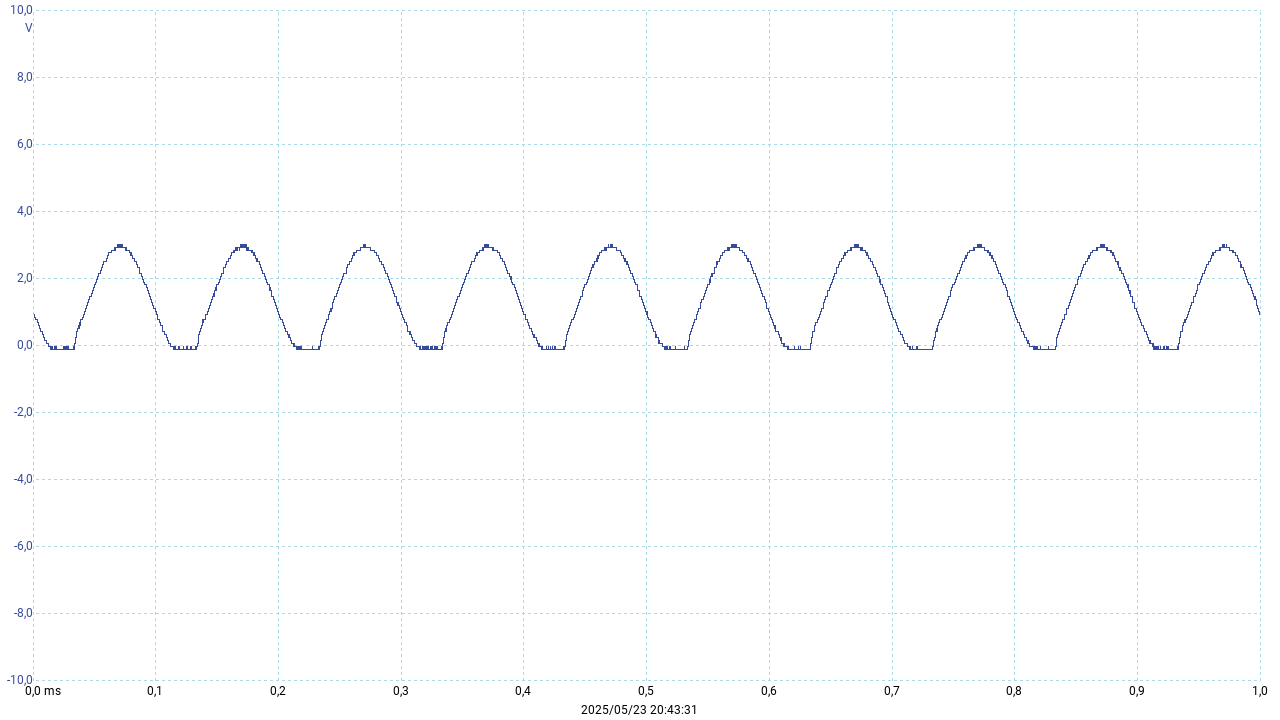
\includegraphics[width=0.95\linewidth]{Figures/Results/scs-output-08Vpp-10kHz}
			\caption{Results showing significant clipping for larger peak-to-peak voltages.}
			\label{fig:scs-output-08Vpp-10kHz}
		\end{subfigure}%
		\begin{subfigure}{.32\textwidth}
			\centering
			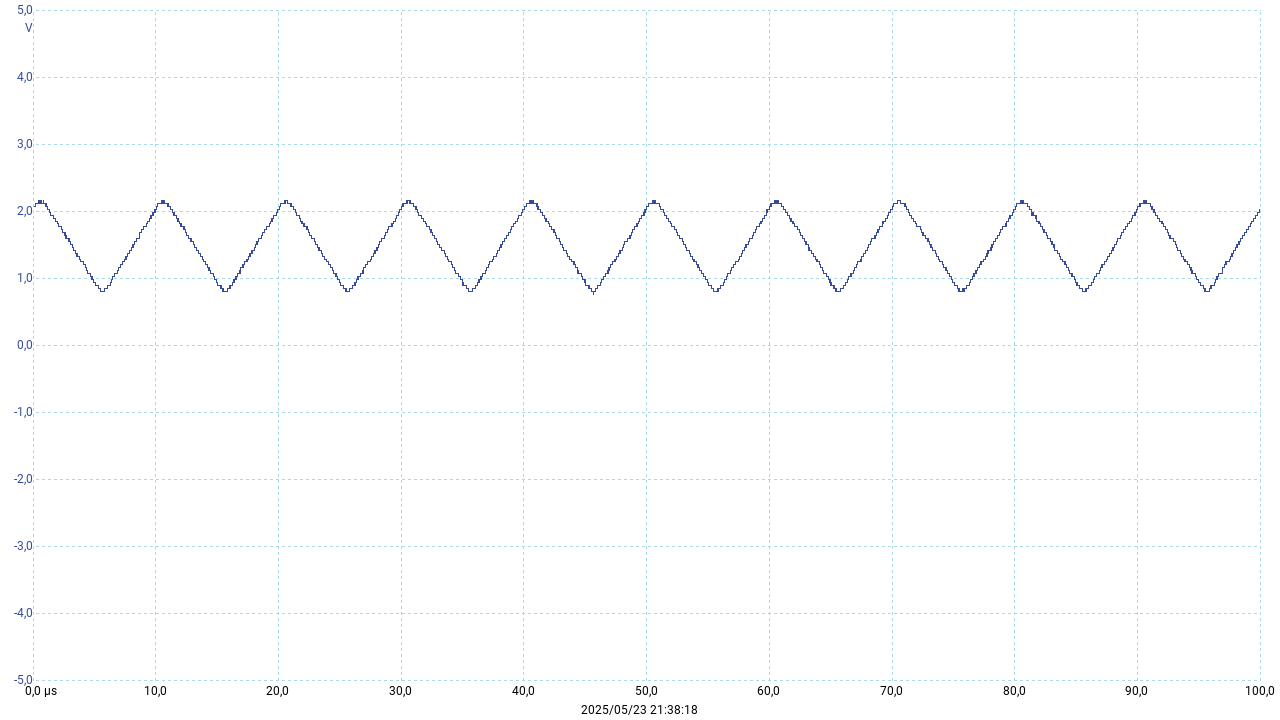
\includegraphics[width=0.95\linewidth]{Figures/Results/scs-output-08Vpp-100kHz}
			\caption{Waveform clipping analysis for a frequency of $\SI{100}{\kilo\hertz}$.}
			\label{fig:scs-output-08Vpp-100kHz}
		\end{subfigure}
		\begin{subfigure}{.32\textwidth}s
			\centering
			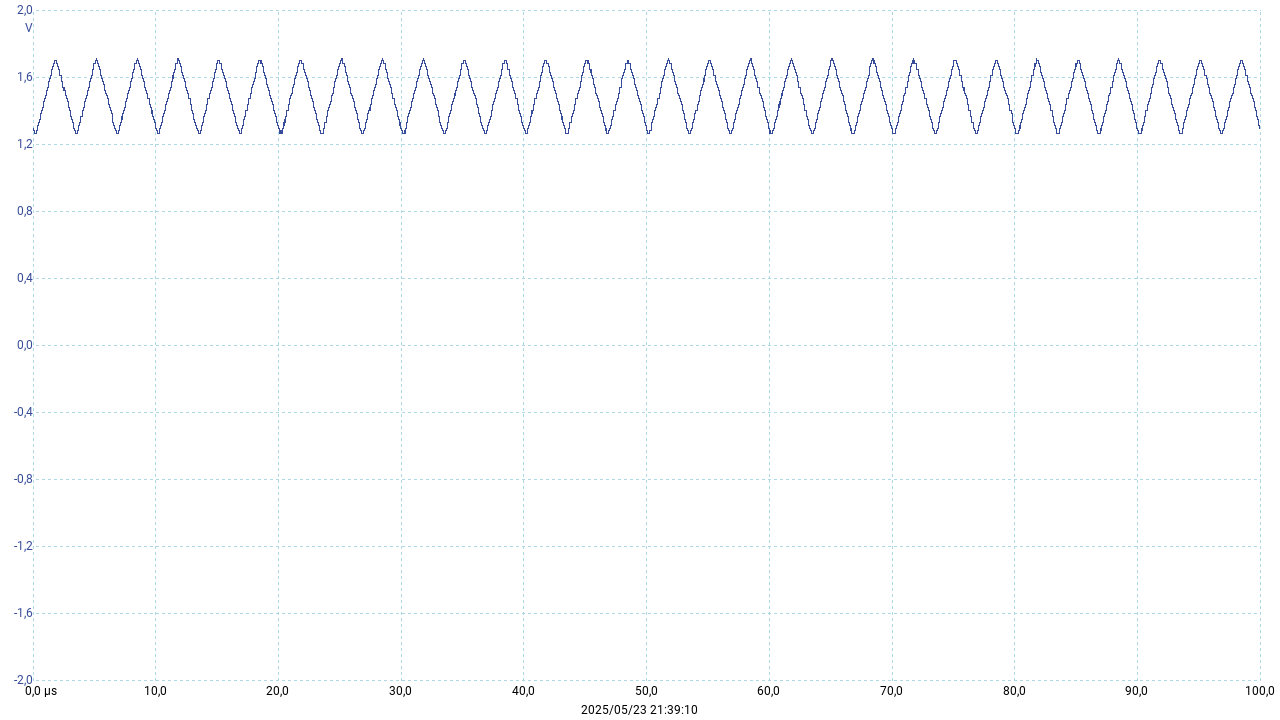
\includegraphics[width=0.95\linewidth]{Figures/Results/scs-output-08Vpp-300kHz}
			\caption{Waveform clipping analysis for a frequency of $\SI{300}{\kilo\hertz}$.}
			\label{fig:scs-output-08Vpp-300kHz}
		\end{subfigure}
		\caption{Results showing the effect of increasing the frequency on the amount of voltage clipping at the output of the \acrshort{scs}.}
		\label{fig:scs-frequency}
	\end{figure} 
	The results show that although clipping is reduced as the frequency is increased, the shape of the output began to collapse to a triangular wave. Additionally, the results in figure \ref{fig:scs-frequency} showed that the peak-to-peak voltage of the \acrshort{scs} output was scaled down and shifted up as the frequency increased. 
	
	Additional results were taken to analyze the response of the subsystem to noisy inputs by supplying a Gaussian noise from the SDG1010. The input Gaussian noise was given a standard deviation of $\SI{136.2}{\milli\volt}$ and a mean voltage of $-\SI{360}{\milli\volt}$ as shown in figure \ref{fig:noisy-vertical}. The \acrshort{scs} showed adequate behaviour because the output voltage was within the range of $\SI{0}{\volt}$ to $\SI{3.3}{\volt}$, as seen in figure \ref{fig:scs-noisy-signal-test}.
	
	\begin{figure}[ht!]
		\centering
		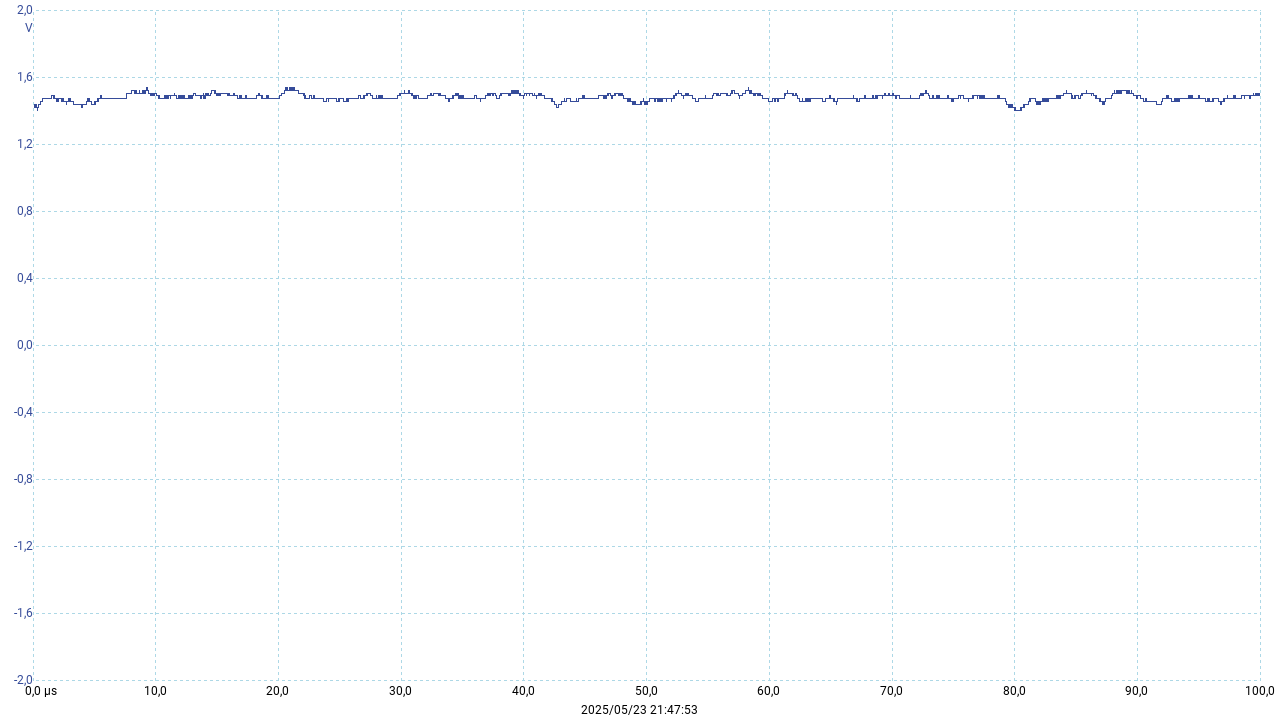
\includegraphics[width=0.55\linewidth]{Figures/Results/scs-noisy-output}
		\caption{Results showing a satisfactory response of the \acrshort{scs} to a noisy vertical input signal.}
		\label{fig:scs-noisy-signal-test}
	\end{figure} 
		
	\begin{table}[ht!]
		\centering
		\begin{tabular}{|c|m{25em}|c|}
			\hline
			\textbf{ID} & \textbf{Description} & \textbf{Outcome} \\
			\hline
			UTC00 & Power the \acrshort{scs} \acrshort{pcb} with a \SI{9}{\volt} supply. Verify that the green LED indicator turns on, confirming power is applied correctly. & Pass \\
			\hline
			UTC01 & Apply a known input to the vertical path. Verify inversion and linear scaling from $-\SI{0.8}{\volt}$ to $\SI{0}{\volt}$ mapped to $\SI{0}{\volt}$ to $\SI{3.3}{\volt}$. & Pass \\
			\hline
			UTC02 & Apply a sawtooth waveform to the horizontal path and confirm that it is linearly scaled from $\pm\SI{5}{\volt}$ to $\SI{0}{\volt}$–$\SI{3.3}{\volt}$ at the output. & Pass \\
			\hline
			UTC03 & Induce a pen-lift event and verify that the signal toggles between \SI{0}{\volt} (scan active) and \SI{3.3}{\volt} (blanking active). & Pass \\
			\hline
			UTC04 & Use high-resolution mode to check for signal ripple. Confirm that peak-to-peak noise remains below \SI{20}{\milli\volt} with no distortion. & Pass \\
			\hline
			UTC05 & Apply out-of-range voltages ($\pm\SI{10}{\volt}$) to inputs. Ensure the output remains clamped and does not exceed safe ADC levels. & Pass \\
			\hline
		\end{tabular}
		\caption{Unit test results for the \acrshort{scs}.}
		\label{tab:scs-unit-tests}
	\end{table}
	
	Outcomes of the unit tests for the subsystem are included in table \ref{tab:scs-unit-test-results}, showing satisfactory behaviour which closely approximates simulated results.
	
	\section{Data Acquisition Subsystem Results}
	
	This section evaluates how reliably the \acrshort{das} converts conditioned analog signals into digital format and stores them in the required \texttt{.csv} structure for downstream processing. Due to the limited availability of the high performance STM32H723ZG microcontroller, the Picoscope 2204A was used as the sampling device in the \acrshort{das}. This was expected to affect the real-time performance of the system. 
	
	To acquire data using the Picoscope, the vertical output of the \acrshort{scs} was connected to channel A while the Picoscope 7 software was opened. While the program running, the \texttt{Save} button was pressed and the file type was set to \texttt{.csv}. The \texttt{.csv} file was saved on the local machine with columns as shown in figure \ref{fig:das-csv}. 
	
	\begin{figure}[ht!]
		\centering
		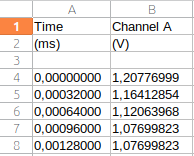
\includegraphics[width=0.35\linewidth]{Figures/Results/das-csv}
		\caption{Showing how data was stored using the Picoscope to generate \texttt{.csv} files for processing in the \acrshort{dsp}.}
		\label{fig:das-csv}
	\end{figure} 
	
	Each \texttt{.csv} file contained 6257 data points, which is sufficient to satisfy the requirement for 801 samples per second. The column with the time-stamps indicated that data points were sampled at intervals of $\SI{0.0003}{\second}$, implying that the sampling frequency of the \acrshort{adc}s on the Picoscope was $\SI{3.3}{\kilo\hertz}$. 
	 
	\section{Digital Processing and Graphical User Interface Results}
	
	This section evaluates the performance of the \acrshort{guis} in terms of visual accuracy, responsiveness, and user experience. Test results include display scaling verification, update latency, and the reliability of interactive controls for switching between display modes. Screenshots and user feedback may be used to support the discussion. Here, the combined behavior of all subsystems is evaluated to assess how well the full digitized HP141T meets its intended purpose. System level outputs are compared with those of the original HP141T to discuss emulation fidelity. Particular focus is placed on real-time performance, mode switching, and overall usability. 
	
	The \acrshort{dps} and \acrshort{guis} were executed based on the \acrshort{rpi} 4B \acrshort{sbc} as shown in figure \ref{fig:rpi-4b-guis}. The \acrshort{rpi} was mounted to the back of the 7 inch touchscreen display and the video cable was connected to both devices. 
	
	\begin{figure}[ht!]
		\centering
		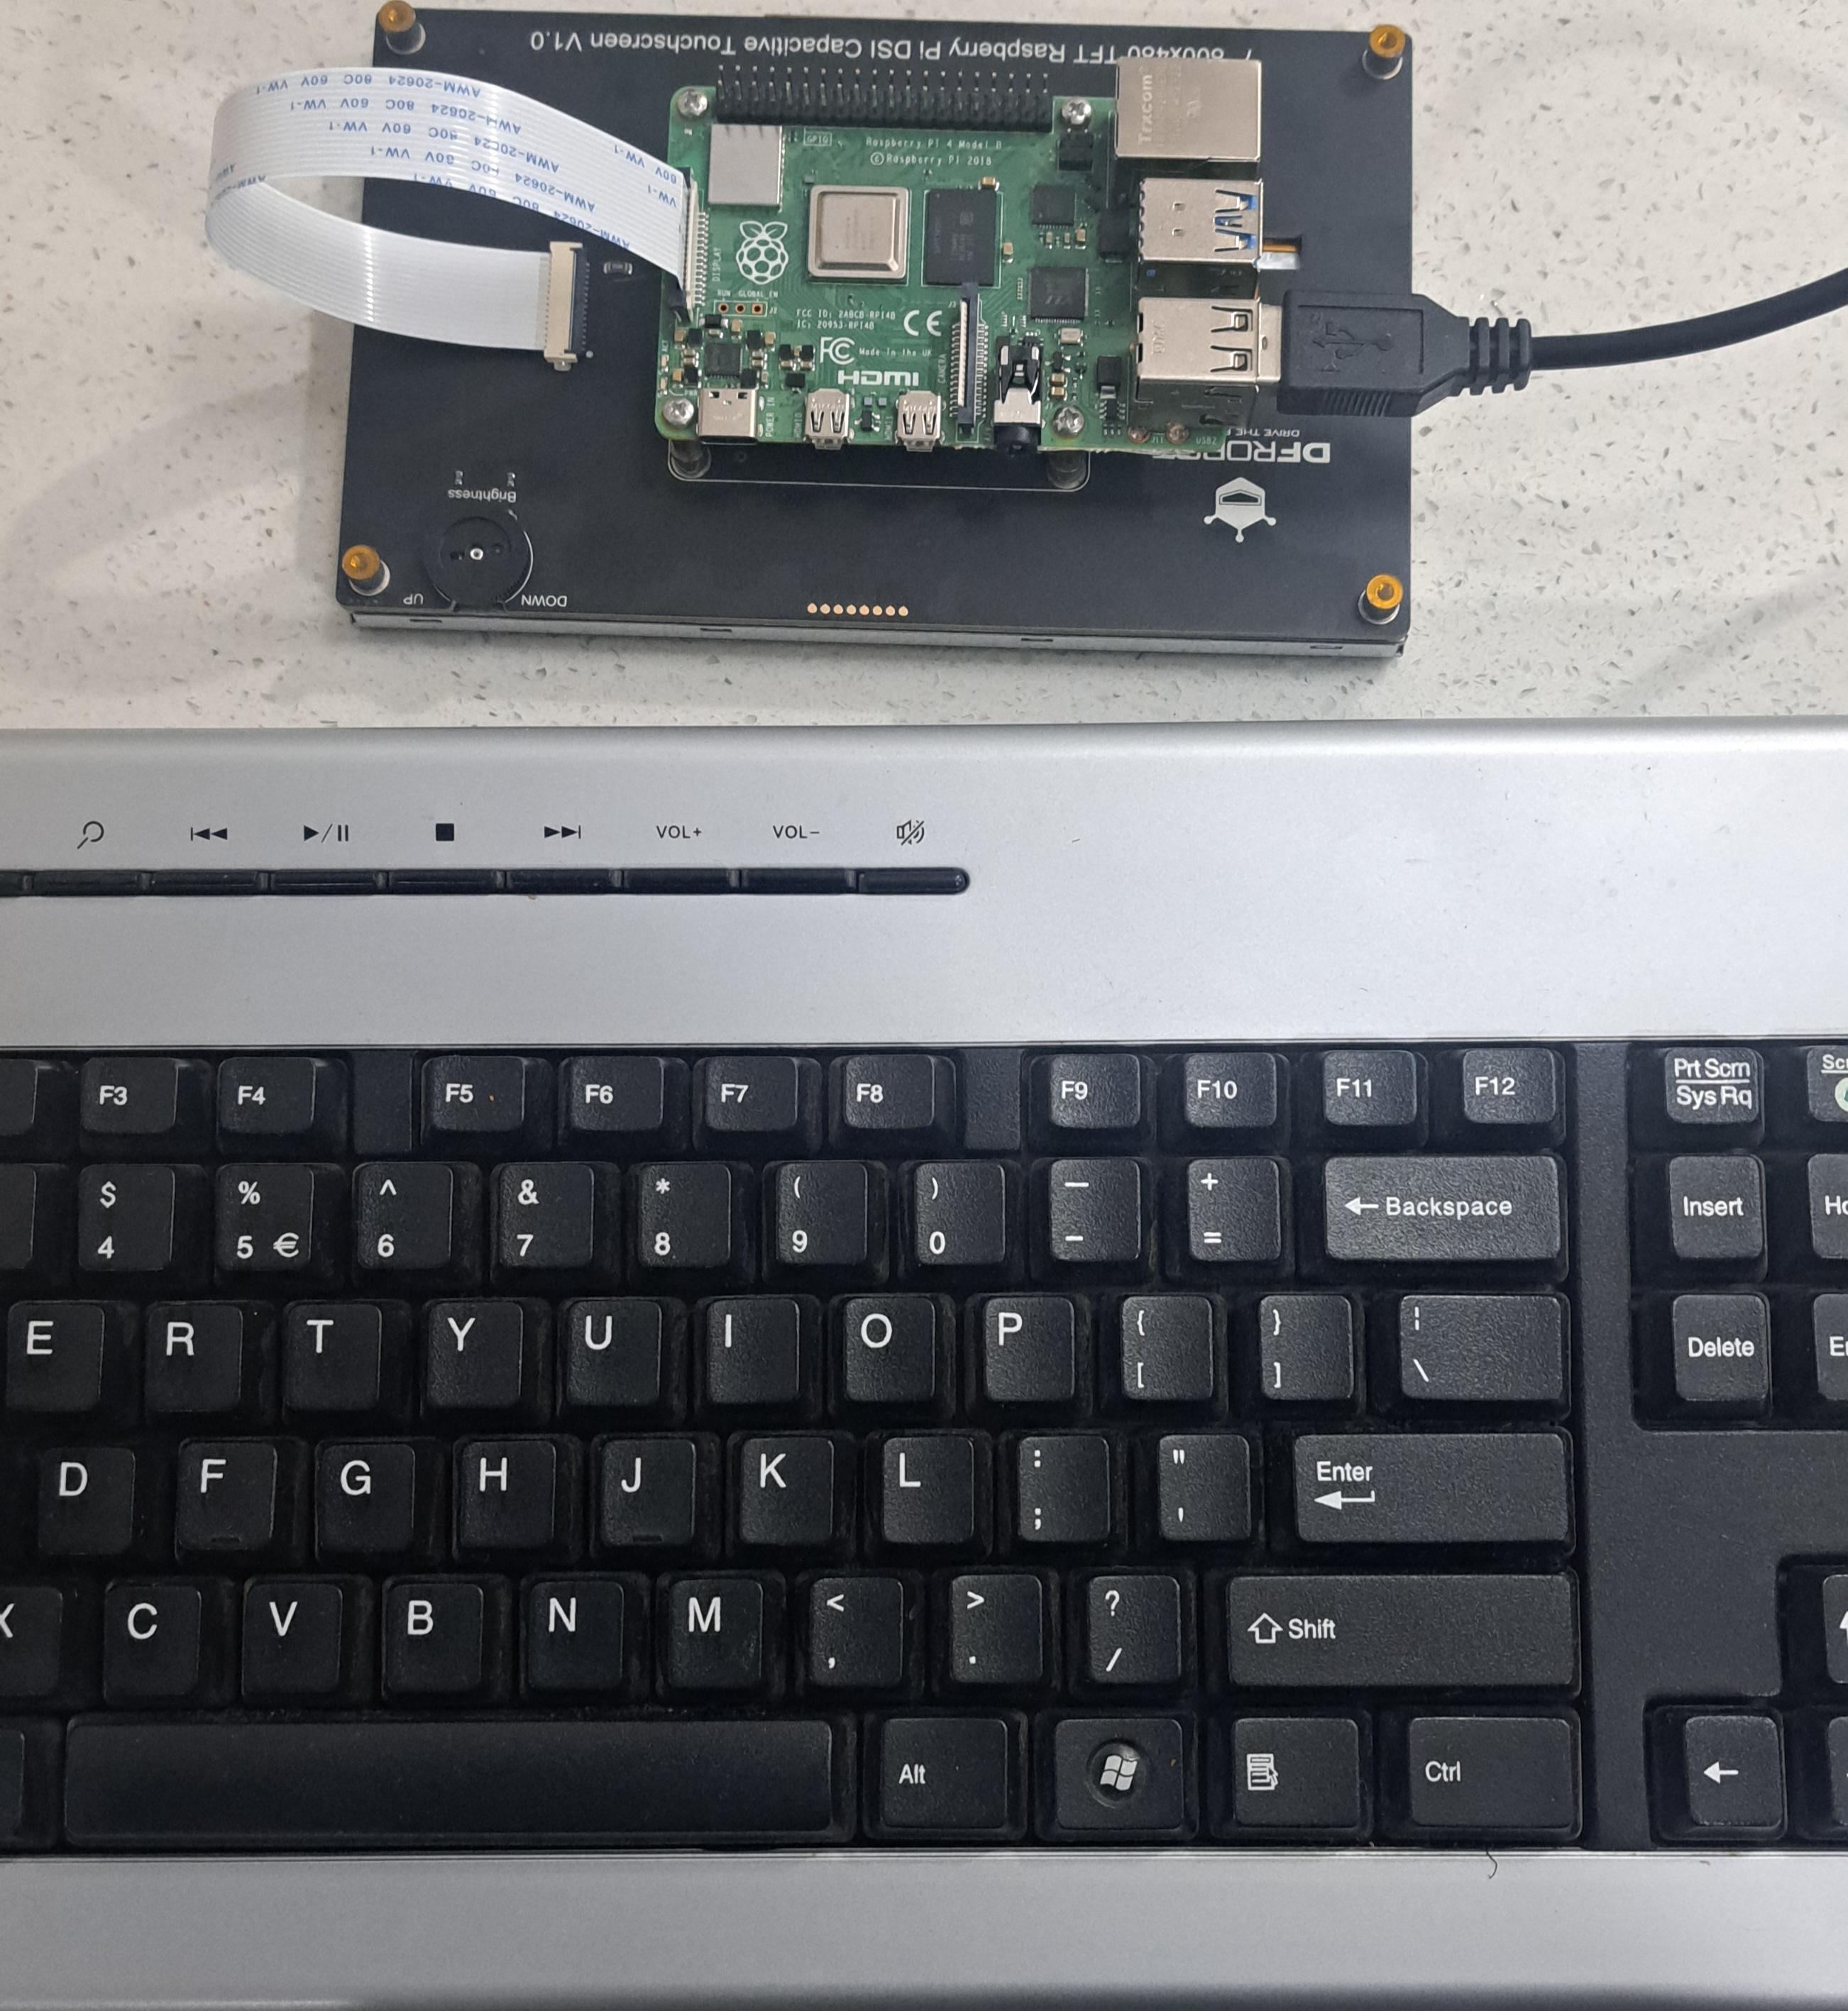
\includegraphics[width=0.35\linewidth]{Figures/Results/rpi-setup}
		\caption{Showing the setup for the \acrshort{dps} and \acrshort{guis} which were both based on the \acrshort{rpi} 4B \acrshort{sbc}.}
		\label{fig:rpi-4b-guis}
	\end{figure} 

	The unit test results for the \acrshort{dps} are shown in table \ref{tab:dps-unit-tests}.
	
	\begin{table}[ht!]
		\centering
		\begin{tabular}{|c|m{25em}|c|}
			\hline
			\textbf{ID} & \textbf{Description} & \textbf{Outcome} \\
			\hline
			UTE00 & Load known values into the DPS and verify that the vertical scaling function correctly converts voltages to dB using the equation $\text{dB} = 80 \times \frac{(3.3 - V_y)}{3.3}$. & Pass \\
			\hline
			UTE01 & Feed multiple spectrograms with varying amplitudes into the DPS. Confirm that the \texttt{max()} function retains the peak amplitude across scans. & Pass \\
			\hline
			UTE02 & Run the \texttt{average\_spectrogram()} function and check that the output bins represent the correct arithmetic mean of all previous values. & Pass \\
			\hline
			UTE03 & Input sparse or irregular data and confirm that the interpolation function fills gaps and produces a smooth, continuous output. & Pass \\
			\hline
			UTE04 & Trace the spectrogram data through the DPS and verify that all values are preserved and correctly passed to the GUI subsystem without corruption. & Pass \\
			\hline
		\end{tabular}
		\caption{Unit test results for the Digital Processing Subsystem (DPS)}
		\label{tab:dps-unit-tests}
	\end{table}

	The unit test results for the \acrshort{guis} are shown in table \ref{tab:guis-unit-tests}.
	
	\begin{table}[ht!]
		\centering
		\begin{tabular}{|c|m{25em}|c|}
			\hline
			\textbf{ID} & \textbf{Description} & \textbf{Outcome} \\
			\hline
			UTF00 & Load decibel values from the DPS and verify that each 10 dB increment corresponds to one vertical division on the GUI plot. & Pass \\
			\hline
			UTF01 & Interact with touchscreen buttons to switch between display modes (e.g., Average, Peak Hold, Raw). Confirm that mode changes are reflected without delay. & Pass \\
			\hline
			UTF02 & Stream spectrogram data to the GUI and confirm that the display updates in near real-time (50–100 ms) with minimal lag. & Pass \\
			\hline
			UTF03 & Load a known dataset and confirm that the GUI plot matches expected amplitude vs frequency output. Check that rendered data aligns with actual values. & Pass \\
			\hline
			UTF04 & Use the pause/resume button during data acquisition and verify that the display halts and resumes without loss of data or state. & Pass \\
			\hline
		\end{tabular}
		\caption{Unit test results for the Graphical User Interface Subsystem (GUIS)}
		\label{tab:gui-unit-tests}
	\end{table}
	
	% ----------------------------------------------------
	\ifstandalone
	\bibliography{../Bibliography/References.bib}
	\printnoidxglossary[type=\acronymtype,nonumberlist]
	\fi
\end{document}
% ----------------------------------------------------